\section{Ageing Well}
\subsection{Summary}

West Sussex is home to 201,000 people aged 65 years or over. Overall, older people in the county are relatively healthy and the county is a good place to live. More people are continuing in paid employment well past the "traditional" retirement age, and older people provide considerable caring support to their families and friends, and the wider community.

The number of older people is projected to increase and to do so at a greater rate than the overall population increase. It will be increasingly important that services, communities and families work together to support older people and their families to remain healthy, happy and at home in the community. To have a healthy older population it is important that the wider determinants of health (housing, planning, income, education etc) are conducive to better ageing, and that organisations and communities work together to promote good health in mid-life, prevent the onset of long- term conditions, and support self-care of health and self-management of conditions.

Overall, health and wellbeing outcomes are good for all life stages in West Sussex, including later life. However, as with the earlier lifestages, the average hides the considerable inequalities in the county.

Life expectancy overall has continued to increase but with healthy life expectancy stalling, this means that more of life is being spent in poor health or with a disability. Male life expectancy still lags behind female life expectancy (80.3 years compared with 83.9 years) and is far lower amongst people from the most deprived and disadvantaged groups, including older people living in poverty and people with a learning disability and/or mental health condition.

The importance of the quality of life lived, not just the length of life, is central to the priorities identified in the West Sussex Health and Wellbeing Strategy 2019-24. Loneliness and social isolation in later life have been identified, through national and local surveys, as impacting the quality of life and are linked to physical health outcomes. Although it should be stressed that the impact of loneliness is not restricted to this age group, it is a life stage when mobility and the opportunity for social contact can decline.

Locally, outcomes relating to falls have fluctuated and often have been poorer compared with comparable authorities; in 2020/21 there were over 4,900 emergency hospital admissions due to falls. At 2,280 per 100,000, this rate is significantly higher than England and the third highest amongst comparable authorities. Of specific concern were the 835 hip fractures in residents aged 80+ years, as, for many older people, such an injury may result in moving into residential care.

Most care is self-care. To self-care and self-manage long-term conditions, people of all ages need access to good advice and may need additional support. Data from the GP Patient Survey found that, across West Sussex, 83\% of people said that they were 'fairly' or 'very' confident in managing their conditions but there is variation across the county and confidence tends to decline with age. In terms of support from local organisations and services, compared to working age adults with a health condition, older people were more likely to say they had enough support.

Just as the quality of birth is valued at the start of life, support for the end of life was identified as a priority by the West Sussex Health and Wellbeing Board. There is again considerable variation across the county; notably, the percentage of people dying at home remains low in Crawley, when compared with the rest of the county and England overall.

\subsection{Over 65 Population Background}
\begin{figure}
    \caption{Year-on-year change in the number of 65+ year olds in West Sussex}\label{fig:over65deltas}
    \centering
    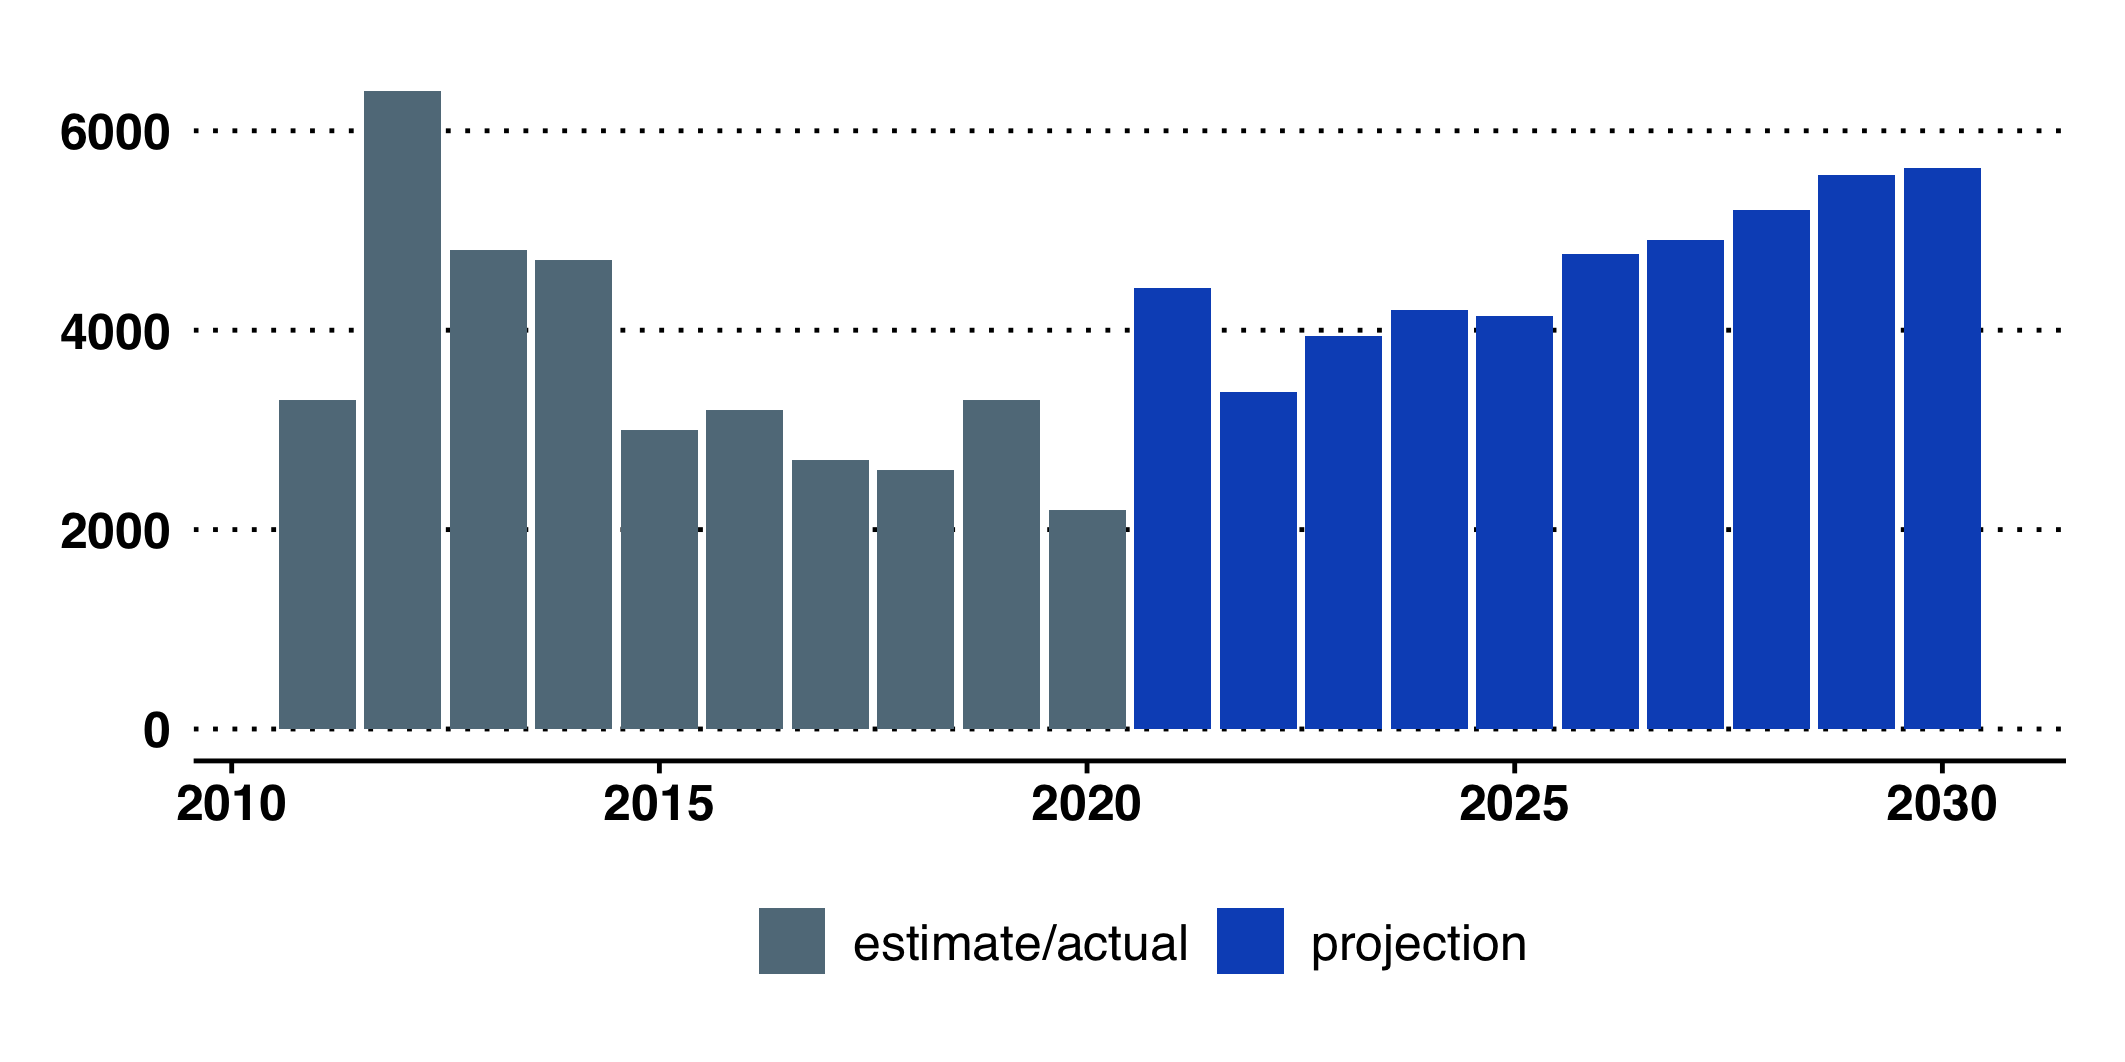
\includegraphics[width=\linewidth]{images/over65_popn_deltas.png}
\end{figure}

\begin{tcolorbox}[title={Population aged 65 years or over}, colback={boxcolour}]
    {\bfseries In 2020, there were an estimated 201,000 people aged 65 years or over in West Sussex,} compared with 164,800 in 2010. In 2030, ONS project that there will be 247,200 people in this age group in West Sussex, with the average year-on-year change increasing from 3,600 in the last 10 years to over 4,500 in the next 10 years.
    
    \begin{itemize}[noitemsep]
        \item Over 30\% of people aged 65 years or over {\bfseries live alone}, representing over 60,000 people and 15\ of all households in West Sussex.
        \item Over 9,100 people aged 65 years or over {\bfseries live in residential or nursing care.}
        \item Over 27,500 people aged 65 years or over are {\bfseries providing unpaid care} for a family member, friend and/or neighbour, with over 9,000 providing unpaid care for 50+ hours a week (and of these, 1,300 are estimated to be aged 85 years or over).%\todo[inline]{Update these figures as per living well chapter}
        \item West Sussex has a {\bfseries high rate of home ownership}, with over 80\% of older people being home owners.
        \item {\bfseries It is estimated that over 40,000 older people (approximately 20\%) in the county have mobility problems} (such as going out of doors and walking down the road; getting up and down stairs; getting around the house on the level; getting to the toilet; getting in and out of bed).
    \end{itemize}
\end{tcolorbox}

\begin{tcolorbox}[title={Loneliness - identifying risks at a neighbourhood level}, colback={boxcolour}]
{\bf Loneliness} is the subjective feeling of a gap between someone's desired and actual social contact. Linked to quality of contacts. Loneliness is not desired by the person experiencing it.

{\bf Social isolation} is an objective measure of contact with others, usually measured in quantitative terms. Some people may choose to have few contacts.

Age UK have produced maps of areas where people may be at greater risk of loneliness. The maps reflect four underlying indicators taken from the 2011 Census: 

\begin{itemize}[noitemsep]
    \item marital status
    \item self-reported health status
    \item age
    \item household size
\end{itemize}

Age UK state that the four factors predicted around 20\% of the loneliness observed amongst people aged 65+. This was established by work undertaken as part of the English Longitudinal Study of Ageing (ELSA). Age UK state that their map should be used alongside local knowledge and understanding of the local population.\footnote{\tiny\url{https://www.ageuk.org.uk/our-impact/policy-research/loneliness-research-and-resources/loneliness-maps/}}
\end{tcolorbox}

%FIGURE - screenshot of the maps in action

\subsection{Long Term Health Conditions}
\paragraph{Older people with long term conditions} Estimates of the number of older people living with a long term condition are based on prevalence assumptions from national research\footnote{The POPPI website from IPC has been used for the estimates.}. Note: these are broad rounded estimates

\begin{itemize}[noitemsep]
    \item People aged 65+ predicted to have {\bfseries diabetes - 25,000}
    \item People aged 65+ estimated to have {\bfseries dementia - 15,100}\footnote{The estimated dementia diagnosis rate in over-65s is a PHOF indicator (E15)}
    \item People aged 65+ predicted to have {\bfseries depression - 17,400}
    \item People aged 65+ predicted to have {\bfseries severe depression - 5,500}
    \item People aged 65+ predicted to have {\bfseries a longstanding health condition caused by bronchitis and emphysema - 3,400}
    %\item People aged 65+ predicted to have a longstanding health condition caused by a stroke - 4,500
    \item People aged 65+ predicted to have {\bfseries a bladder problem at least once a week - 33,500}
    \item People aged 65+ predicted to have {\bfseries a fall - 54,700}
    \item People aged 65+ predicted to be {\bfseries admitted to hospital as a result of a fall - 6,700}
    \item People aged 65+ predicted to have {\bfseries severe hearing loss - 16,700}
    % \item People aged 75+ predicted to have registrable eye conditions - 6,200 % Apparently this isn't in POPPI, but could refer to the West Sussex SINA instead?
\end{itemize}

In relation to recorded prevalence, approximately 6,368 people in West Sussex are on GP dementia registers.

%, the majority (over 5,700) in the Coastal West Sussex CCG area.
% NB - could look for PCNs with highest and lowest recorded dementia prevalence

\paragraph{Musculoskeletal problems (MSK)} In 2021, {\bfseries 16.4\% of people aged 18+ reported a long-term Musculoskeletal (MSK) problem}\footnote{PHOF reference C27}, such as a long-term back pain or joint pain, representing over 116,900 people in West Sussex. This is similar to England (17\%).

\paragraph{Sensory impairment} Independence in later life can be severely impacted by hearing and sight loss. Sensory impairment can act to increase loneliness and social isolation and hearing loss is a risk factor for dementia at older ages.

\begin{itemize}
    \item Around 18,000 people aged 65 years or over are estimated to have a moderate to severe visual impairment\footnote{Visual acuity (VA) of less than 6/18 (moderate or severe) is largely used as the point which approximates to the statutory threshold for qualifying as registered severely sight impaired (blind) or registered sight impaired (partially sighted).}. Of those over 75 years, approximately half are estimated to have "correctable sight loss", with conditions such as cataracts.
    \item 6,200 people aged 75 years or over are estimated to have a registrable eye condition.
    \item 17,000 people aged 65 years or over are estimated to have severe hearing loss\footnote{Hearing loss is measured by assessing the quietest sounds someone can hear using tones with different frequencies. In hearing tests, a person is asked to indicate when they can hear a tone; the level is then adjusted to find their threshold, when they can just hear it. Thresholds are measured in units called dBHL: dB stands for 'decibels' and HL stands for 'hearing level'. The greater the threshold level in dBHL, the worse the hearing loss. People with thresholds between 0 and 20 dBHL across all the frequencies are considered to have 'normal' hearing. The threshold of 25 dBHL indicates some hearing loss; the threshold of 65 dBHL indicates severe hearing loss. (adapted from POPPI Source: IPC)}.
    \item {\bfseries Sight loss due to age-related macular degeneration (AMD) in 65+ year-olds has decreased in West Sussex in the last three years}. In 2020/21, the rate in West Sussex was 70.1 per 100,000 and, having previously been higher than England, is now below the national rate and is ranked eleventh amongst comparable local authorities. In 2020/21, there were 141 new Certifications of Visual Impairment (CVI), 37 fewer than 2020/21.
\end{itemize}

%{\bf Preventable sight loss - age related macular degeneration (AMD)}

\begin{figure}
    \caption{Rate of new Certifications of Visual Impairment per 100,000 over-65s in West Sussex}\label{fig:amd_wsx}
    \centering
    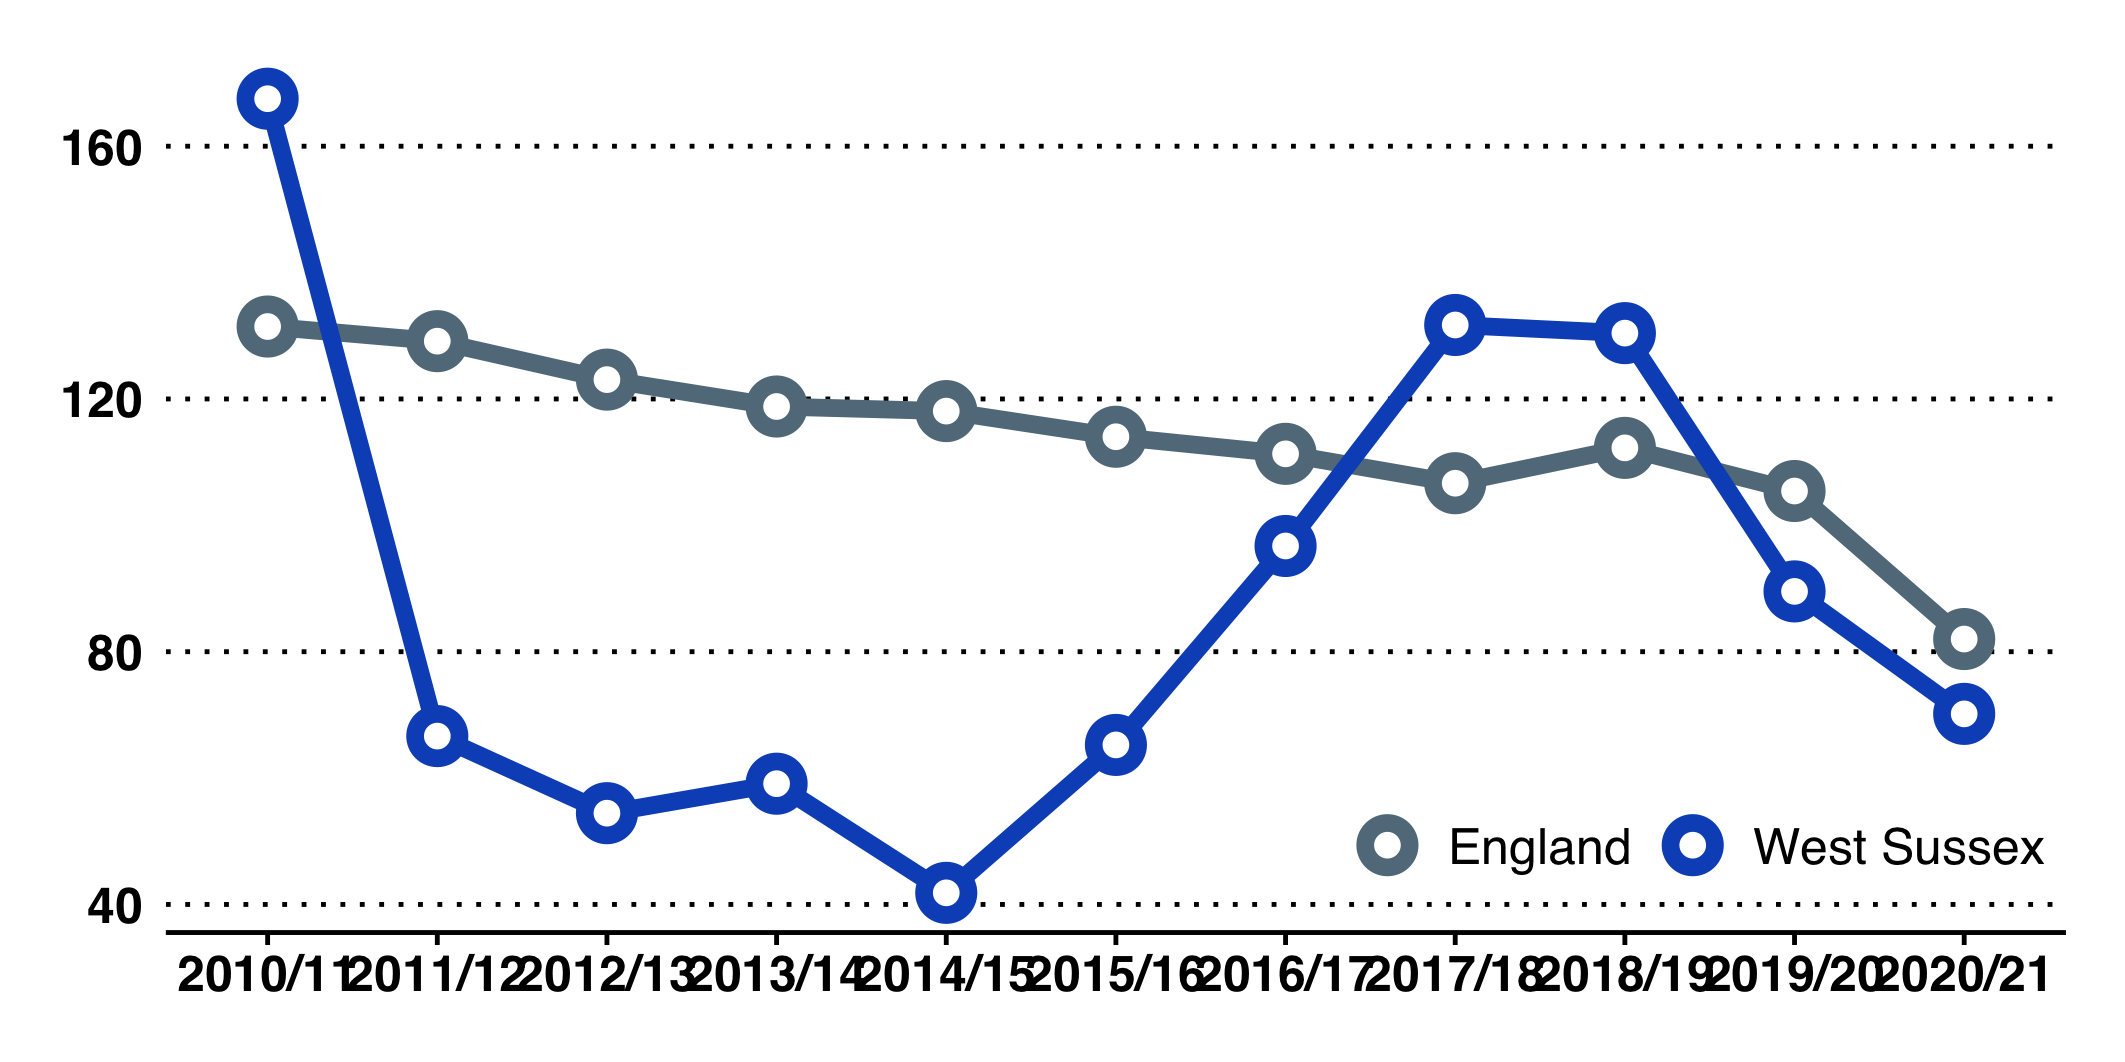
\includegraphics[width=\linewidth]{images/amd_line.png}
\end{figure}

\subsection{Multi-morbidity estimates}
\paragraph{Multi-morbidity - Public Health England Estimates} As we age we are likely to have or develop one or more long term health condition. This is called co-morbidity.

In 2018, Public Health England (as was) published estimates of the number of people with multi-morbidities in each lower tier authority in England. In doing this, PHE noted some challenges in how multi-morbidity is described, including how many and which conditions are included (physical and/or mental health conditions).

The physical conditions included in the PHE estimates are listed in Table~\ref{tab:op:phys_conditions} on page~\pageref{tab:op:phys_conditions}. The mental health conditions are listed in Table~\ref{tab:op:mh_conditions} on page~\pageref{tab:op:mh_conditions}.

\begin{table*}
    \caption{Physical Conditions included in the PHE Estimates}
    \centering
    \begin{tabular}{ccc}
        \toprule
        Hypertension & Heart failure & Treated constipation\\
        Painful condition & Prostate disorders & Stroke \& transient Ischaemic attack\\
        Asthma (currently treated) & Glaucoma & Chronic kidney disease \\
        Coronary heart disease & Epilepsy (currently treated) & Diverticular disease of intestine \\
        Treated dyspepsia & Psoriasis or eczema & Viral Hepatitis \\
        Diabetes & Inflammatory bowel disease & Chronic liver disease \\
        Thyroid disorders & Migraine & Atrial fibrillation \\
        Rheumatoid athritis & Blindness \& low vision & Peripheral vascular disease \\ 
        Hearing loss & Chronic sinusitis & Parkinson's disease \\
        Chronic obstructive pulmonary disease & Irritable bowel syndrome & Multiple sclerosis \\
        Bronchiectasis & New diagnosis of cancer in last 5 years & \ \\
        \bottomrule
    \end{tabular}
    \label{tab:op:phys_conditions}
\end{table*}
\begin{table*}
    \caption{Mental Health Conditions included in the PHE Estimates}\
    \centering
    \begin{tabular}{ccc}
        \toprule
        Anorexia or bulimia & Anxiety \& other neurotic, stress & Schizophrenia (and related non-organic psychosis) \\
        \ & related \& somatoform disorders & or bipolar disorder \\
        Depression & Learning disability & Dementia \\
        Alcohol problems & \ & \ \\
        \bottomrule
    \end{tabular}
    \label{tab:op:mh_conditions}
\end{table*}
  
\subsubsection{Multi-morbidity estimates by age - West Sussex}

Tables~\ref{tab:op:2_plus_conds}~through~\ref{tab:op:m_and_p} show the multimorbidity estimates from PHE applied to 2020 population estimates.

\begin{table}
    \caption{Multi-morbidity estimates by age - West Sussex. Prevalence of 2 or more chronic conditions applied to 2020 population estimates.}
    \centering
    \begin{tabular}{lrr}
        \toprule
        \ & Number & Prevalence \\
        \midrule
        0-24 years & 4,090 & 1.7\% \\
        25-44 years & 21,940 & 11.1\% \\
        45-64 years & 70,210 & 29.5\% \\
        65-84 years & 109,720 & 64.2\% \\
        85+ years & 24,500 & 81.4\% \\
        \bottomrule
    \end{tabular}
    \label{tab:op:2_plus_conds}
\end{table}

\begin{table}
    \caption{Multi-morbidity estimates by age - West Sussex. Prevalence of 3 or more chronic conditions applied to 2020 population estimates.}
    \centering
    \begin{tabular}{lrr}
        \toprule
        \ & Number & Prevalence \\
        \midrule
        0-24 years & 720 & 0.3\% \\
        25-44 years & 8,300 & 4.2\% \\
        45-64 years & 36,410 & 15.3\% \\
        65-84 years & 75,370 & 44.1\% \\
        85+ years & 19,440 & 64.6\% \\
        \bottomrule
    \end{tabular}
    \label{tab:op:3_plus_conds}
\end{table}

\begin{table}
    \caption{Multi-morbidity estimates by age - West Sussex. Physical \& Mental health co-morbidity prevalence applied to 2020 population estimates.}
    \centering
    \begin{tabular}{lrr}
        \toprule
        \ & Number & Prevalence \\
        \midrule
        0-24 years & 1,200 & 0.5\% \\
        25-44 years & 10,870 & 5.5\% \\
        45-64 years & 27,610 & 11.6\% \\
        65-84 years & 28,540 & 16.7\% \\
        85+ years & 9,090 & 30.2\% \\
        \bottomrule
    \end{tabular}
    \label{tab:op:m_and_p}
\end{table}

% \clearpage

\subsection{Segmenting the 65+ Population}
\subsubsection{Using GP Patient Register Data}
Registered patient data provide details of age, sex, long-term conditions (nature of condition and number), and may include some data on health care activity and cost. Public Health has some, but limited, access to the data. We have been able to analyse anonymised data to provide a population level view of a health and to segment the 65+ population. The intelligence provided by the sample of records (approximately 30\% of the West Sussex 65+ population).

The data show that {\bfseries 54\% of patients at age 65 had no long term health condition}, but that {\bfseries this falls to 21\% by the age of 85 years}. Using sample data\footnote{All patients registered with Crawley, Horsham and Mid Sussex CCG GPs in 2015, excluding people identified as living in a care homes (2.2\% of the sample)}, it was found that of the population aged 65 years and over: 
\begin{itemize}[noitemsep]
    \item 62.7\% had no or 1 long term condition (hypertension was the most common, see Figure~\ref{fig:gprd_seg_ltc} on page~\pageref{fig:gprd_seg_ltc}.)
    \item 26.6\% had 2 or 3 conditions
    \item 8.5\% had 4 or more conditions
\end{itemize}

%FIGURE - Age and the Number of Long Term Conditions (LTCs) (Based on data from Crawley, Horsham and Mid Sussex) (graph)
\begin{figure}[H]
\caption{Specific Conditions and percentage of Age Group Identified with Long Term Conditions}\label{fig:gprd_seg_ltc}
\centering
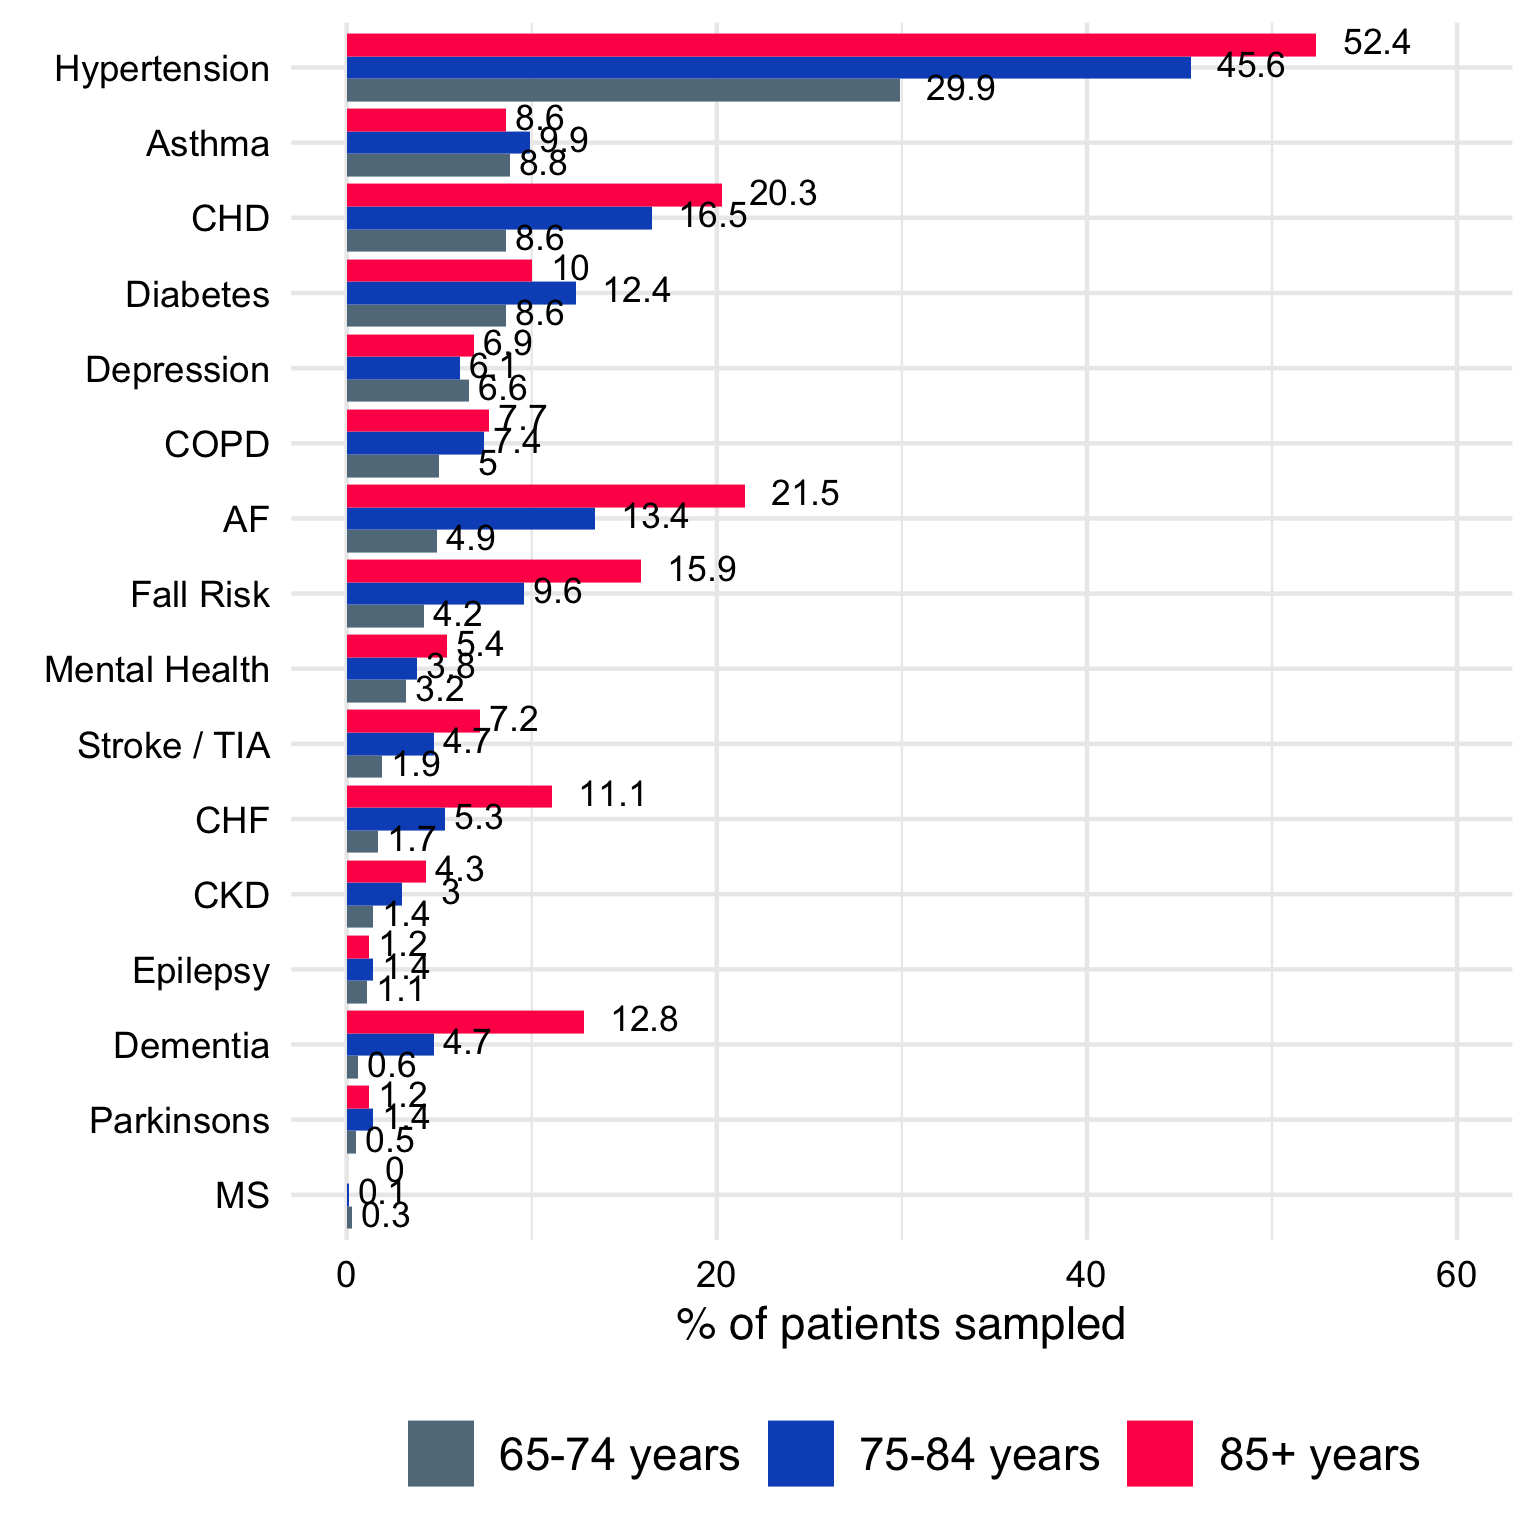
\includegraphics[width=\linewidth]{images/GPRD_seg_ltc.png}
\end{figure}

\newpage

\subsubsection{Estimating Care Needs in a Population}
In 2020, there were an estimated 201,000 residents in West Sussex aged 65 years or over. To help plan services for older people, different approaches can be used to estimate how many older people (in any year) may need help to maintain or regain independence, and how many may need on-going support from others. To do this, we segment residents into distinct groups. There are various ways to estimate these groups. Using different datasets, three methods are set out in our briefing document available on the JSNA website and summarised below.

In any one year, residents may fall into one of four scenarios/segments:

\begin{itemize}[noitemsep]
    \item {\bf Independent} - Most people aged 65+ are "fully" independent and need no formal (paid) support
    \item {\bf Short-term/Regain} - Some people need temporary support (for example after a fall or a short term illness)
    \item {\bf On-going} - Some people need on-going and long term support, in the community or in residential care
    \item {\bf Die} - Estimated number of people aged 65+ (in total) that die each year
\end{itemize}

Three methods of segmenting the population were considered:

\begin{itemize}[noitemsep]
    \item using population health data from the census
    \item using  assumptions about the need for support to undertake activities for daily living
    \item using the prevalence of people with long-term health conditions
\end{itemize}

Table~\ref{tab:care_segments} (on page~\pageref{tab:care_segments}) shows the approximate number of older people in each segment based on 2020 population estimates.

\begin{table}[H]
    \caption{Segmentation of West Sussex population aged 65+ according to likely care needs based on 2020 population estimates.}
    \centering
    \begin{tabular}{lrrrr}
        \toprule
        \ & Independent & Short-term / Regain & Ongoing & Death \\
        \midrule
        Method 1 & 118,100 & 34,100 & 34,100 & 8,300\\
        Method 2 & 135,600 & 34,400 & 22,500 & 8,300\\
        Method 3 & 120,800 & 51,200 & 20,700 & 8,300\\
        \bottomrule
    \end{tabular}
    \label{tab:care_segments}
\end{table}

\subsection{Self care} 
The Self Care Forum\footnote{http://www.selfcareforum.org/} provides a range of resources relating to self-care and have conceptualised self-care as a continuum from decisions made everyday to managing long term conditions.

\begin{figure}
    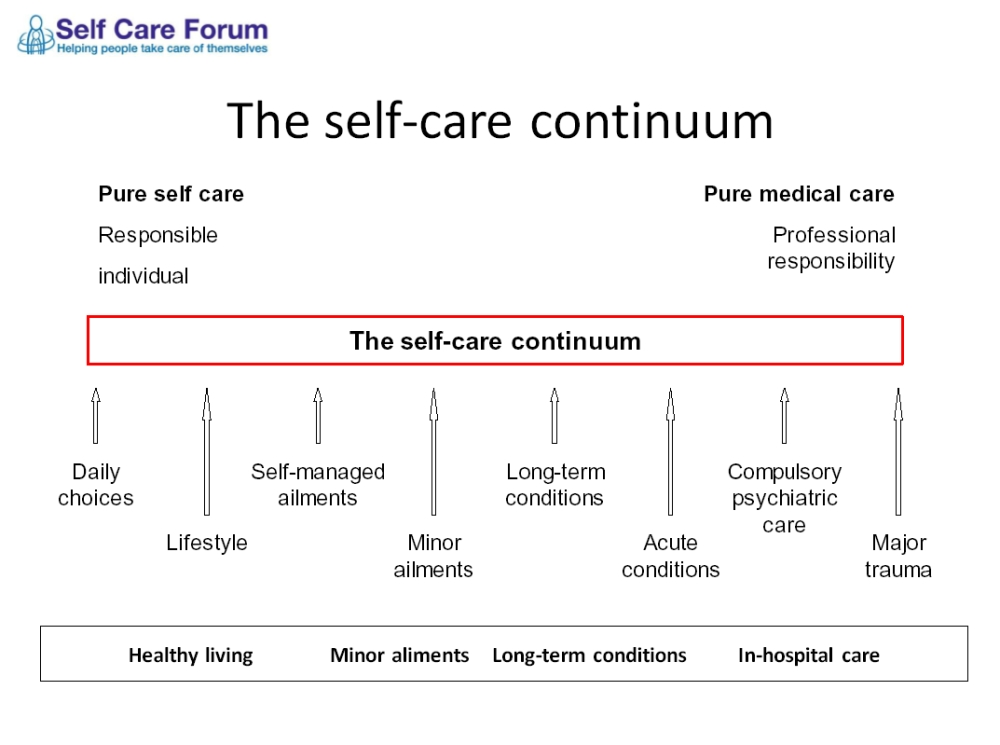
\includegraphics[width=\linewidth]{images/04-self-care-continuum.jpeg}
\end{figure}

As people age, general health declines and the likelihood of having one or more long-term health condition or disability increases. {\bfseries It should be recognised that most care in a society is "informal": self-care, or care provided by others in a family or group of friends and neighbours.} One source of self-care data is the GP Patient Survey, which includes the following questions:

\begin{itemize}[noitemsep]
    \item How confident are you that you can manage any issues arising from your condition (or conditions)?
    \item In the last 12 months, have you had enough support from local services or organisations to help you to manage your condition (or conditions)?
\end{itemize}

Data for West Sussex overall for 2019 are shown below. GP Patient Survey data are available at CCG and individual practice level, although care should be taken with small sample sizes\footnote{Data can be accessed and analyzed at \url{https://gp-patient.co.uk/}}.

\paragraph{Confidence in managing condition(s)} 86\% of people overall said they were fairly or very confident in managing their health condition. This declines with age; within the 85+ years respondent group, 1 in 3 said their were not very or not at all confident.

\begin{figure}
    \caption{Confidence in managing long term conditions - 2021 GP Patient Survey, West Sussex CCG.}\label{fig:gpps_ltc_confidence}
    \centering
    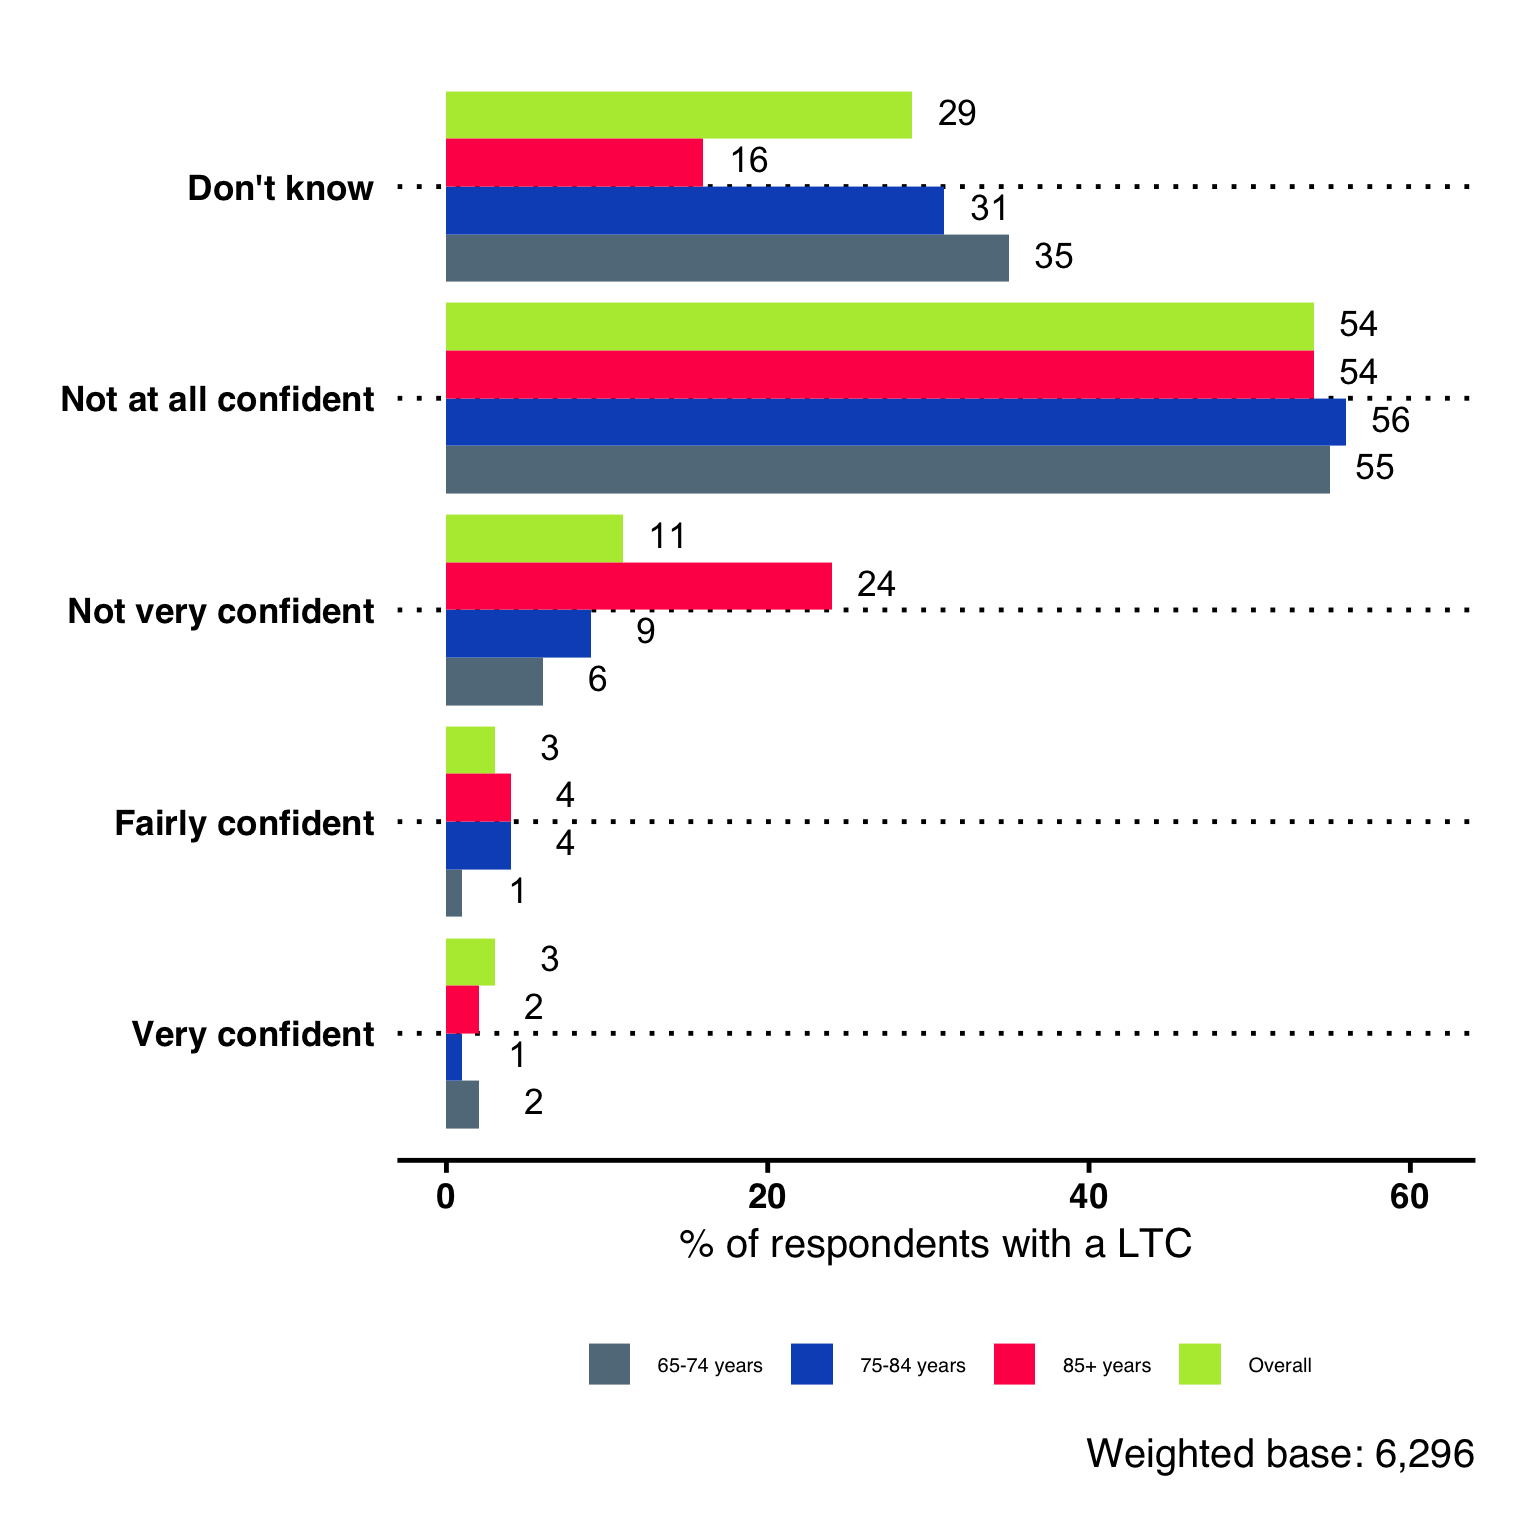
\includegraphics[width=\linewidth]{images/GPPS_confident_LTC.png}
\end{figure}

\begin{figure}
    \caption{Responses to the question "Do you feel you have enough support from local services and organisations?" 2021 GP Patient Survey, West Sussex CCG.}\label{fig:gpps_support}
    \centering
    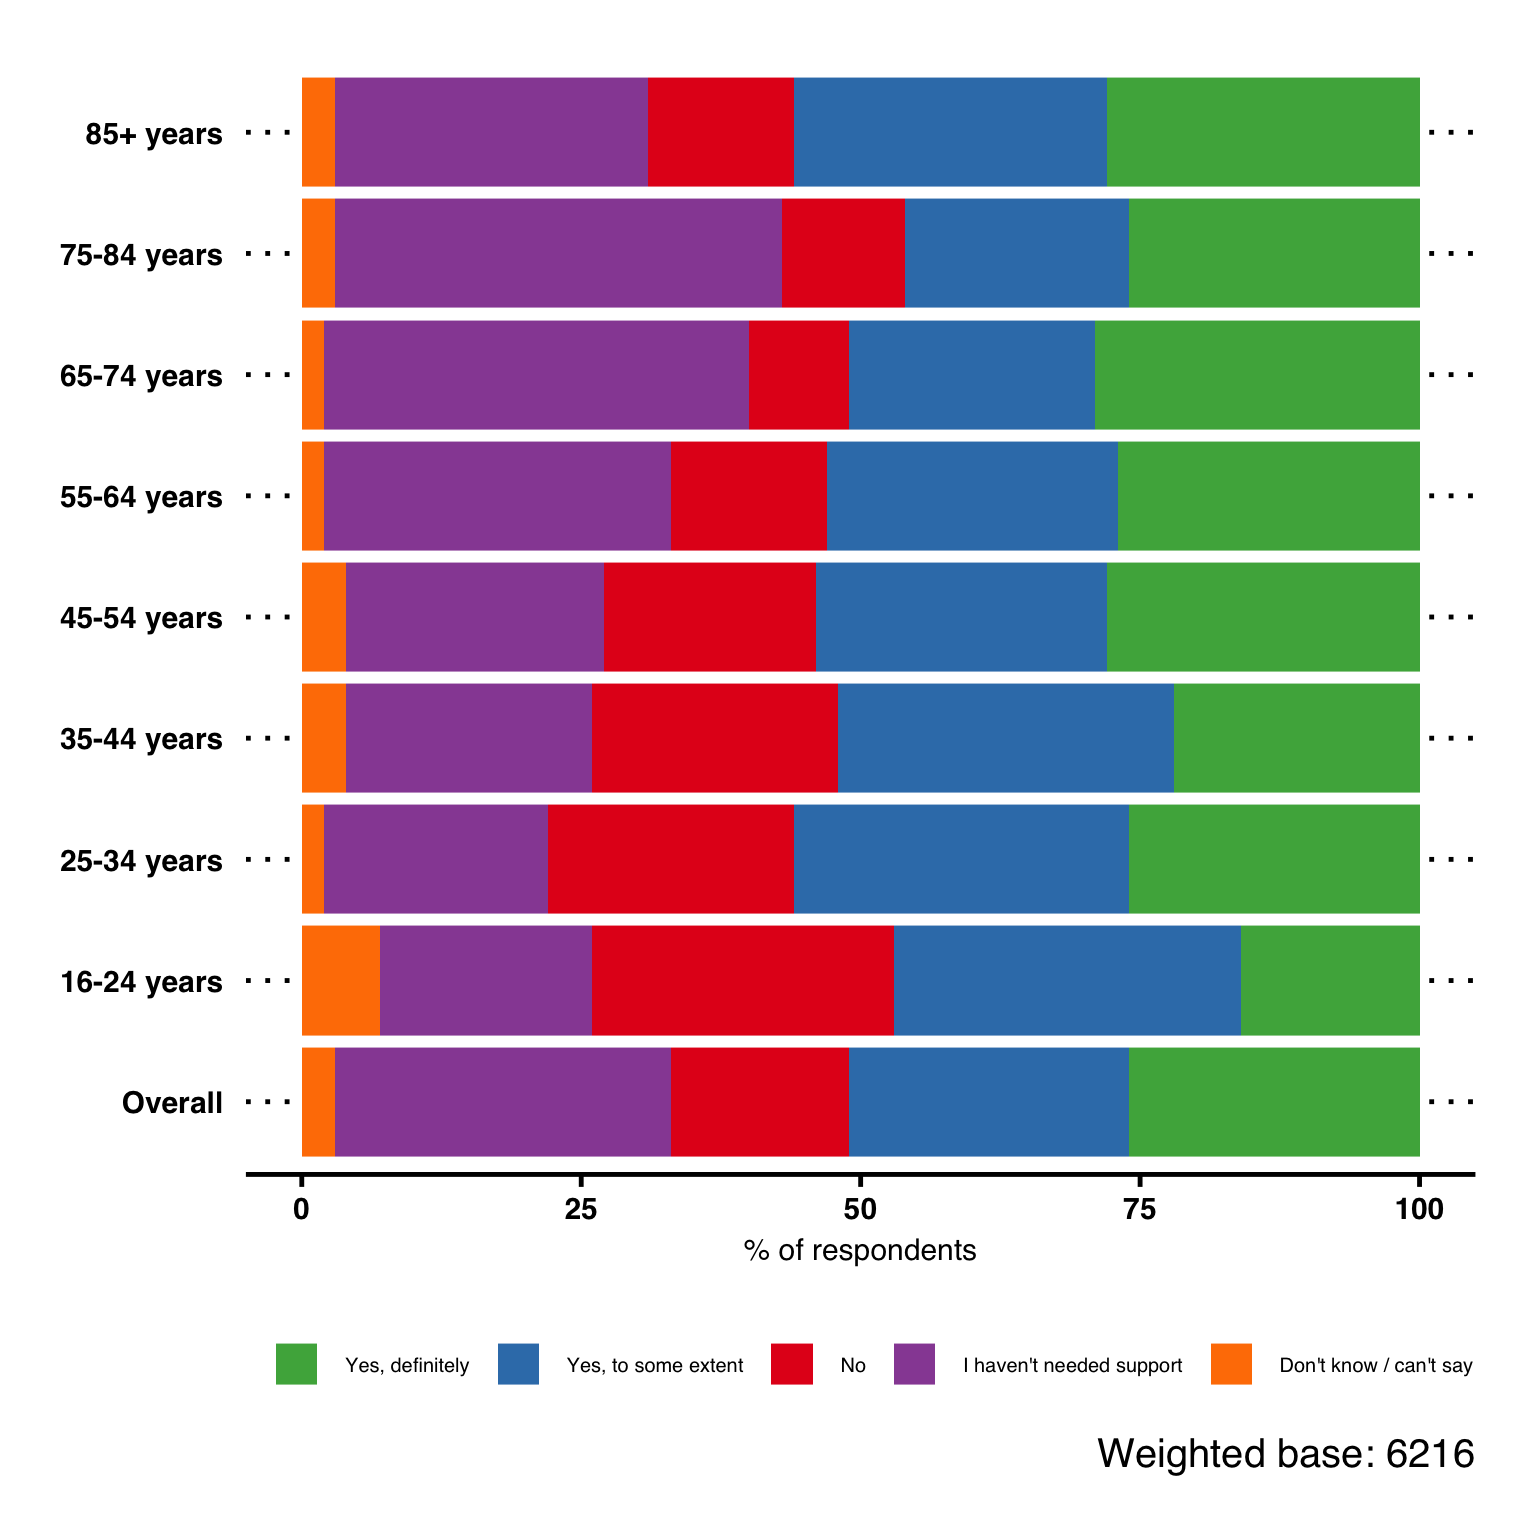
\includegraphics[width=\linewidth]{images/GPPS_support.png}
\end{figure}


\paragraph{Enough support from local services and organisations to help manage condition(s)} 
\begin{itemize}
    \item A higher percentage of people with a long-term condition who said they have not had enough support were of the working age-groups, compared to the older age-groups.
    \item 1 in 4 respondents aged 16-24 years with a long term health condition said they have not had enough support from local services and organisations.
\end{itemize}

\subsection{Social Care - Expressed Demand}
\subsubsection{Need Related to Activities of Daily Living}
Most people who have care needs do not seek or obtain support from statutory organisations. On the next few pages, published comparable data are shown in relation to people who request and/or are in receipt of support from West Sussex County Council.

A wide range of data are available, and published by NHS Digital \url{https://digital.nhs.uk/data-and-information/areas-of-interest/social-care}

In interpreting this information some care should be taken, especially where there are large year-on-year fluctuations. These may reflect changes in definition (or interpretation of definitions) or underlying issues of data collection.

\subsubsection{Route of Access - New Clients (Excluding Repeat Requests)}
\begin{itemize}[noitemsep]
    \item 96\% of new requests from 18-64 year-olds and 81\% of requests from 65+ year-olds came from the community, which is higher than the national percentages.
    \item For 65+ year-olds, 15\% came from hospital discharge in 2020/21.
    \item For 18 - 64 year-olds, very few requests into adult social care are recorded as planned transitions.
    \item For both age groups, the 'other' category in these numbers includes capital depleters, hospital diversions, prison and planned (transition). 
\end{itemize}

\begin{figure*}
    \caption{New requests for social care in West Sussex.}\label{fig:sc-requests}
    \vspace*{5mm}
    \centering
    \begin{subfigure}[b]{0.49\textwidth}
        \centering
        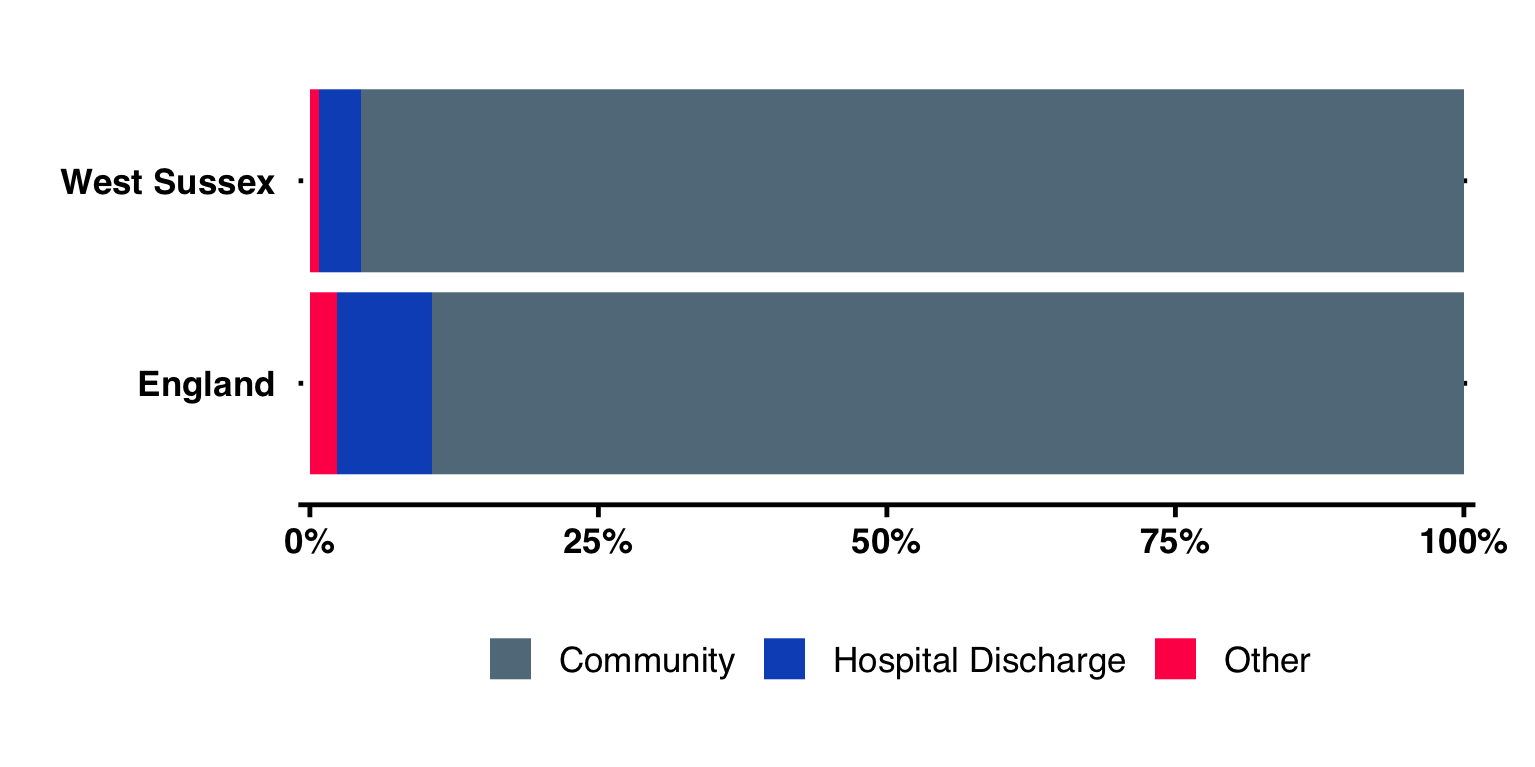
\includegraphics[width=\textwidth]{images/new_sc_requests_18_to_64.png}
        \caption{New social care requests from 18-64 year olds, West Sussex and England, 2020/21.}
        \label{fig:sc:new_requests_18_64}
    \end{subfigure}
    \begin{subfigure}[b]{0.49\textwidth}
        \centering
        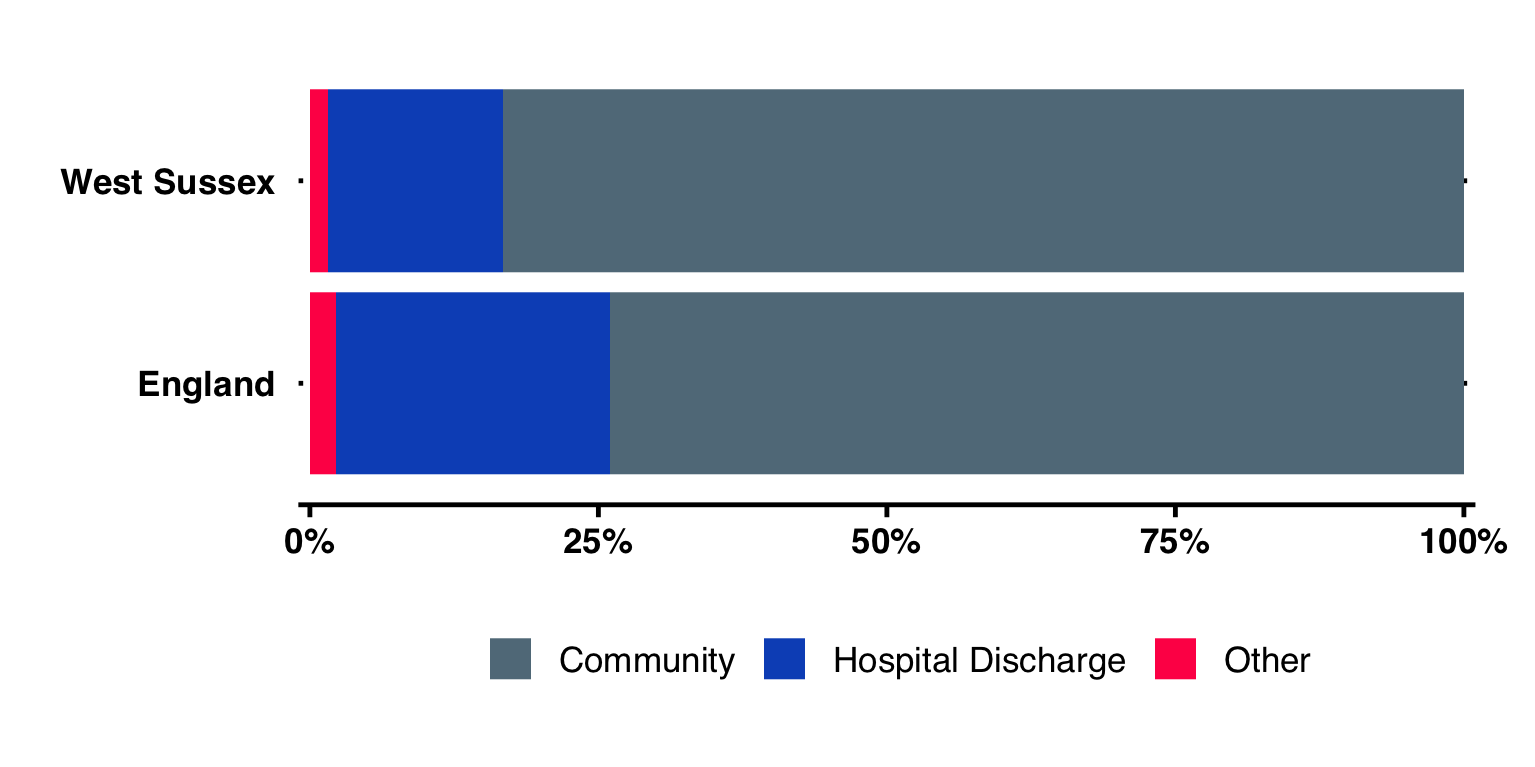
\includegraphics[width=\textwidth]{images/new_sc_requests_65_plus.png}
        \caption{New social care requests from 65+ year olds, West Sussex and England, 2020/21.}
        \label{fig:sc:new_requests_65_plus}
    \end{subfigure}
    \begin{subfigure}[b]{0.49\textwidth}
        \centering
        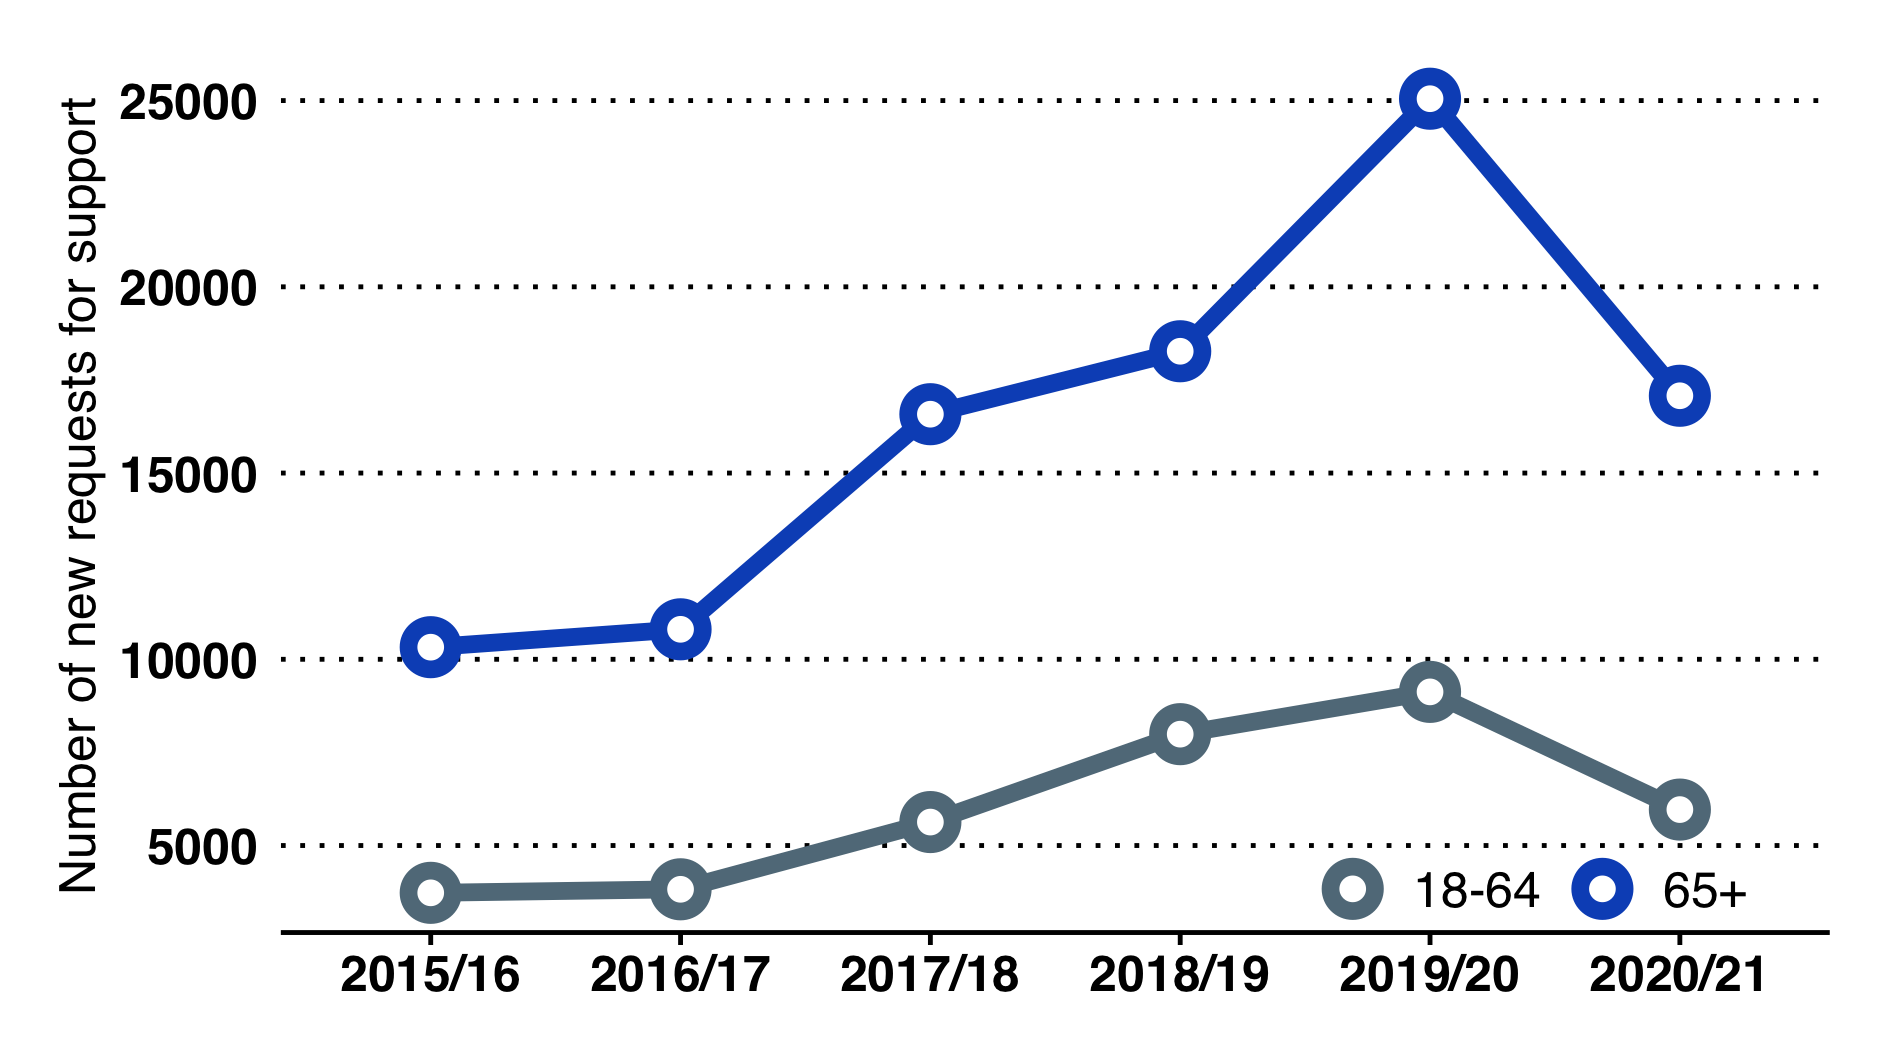
\includegraphics[width=\textwidth]{images/new_sc_requests_line.png}
        \caption{Number of new requests to social care by age, West Sussex and England, 2016/17 to 2020/21.}
        \label{fig:sc:number_of_requests_by_age}
    \end{subfigure}
\end{figure*}

\begin{figure*}
    \caption{Demand for social care over time, West Sussex compared to England.}\label{fig:more-sc-requests}
    \vspace*{5mm}
    \centering
    \begin{subfigure}[b]{0.49\textwidth}
        \centering
        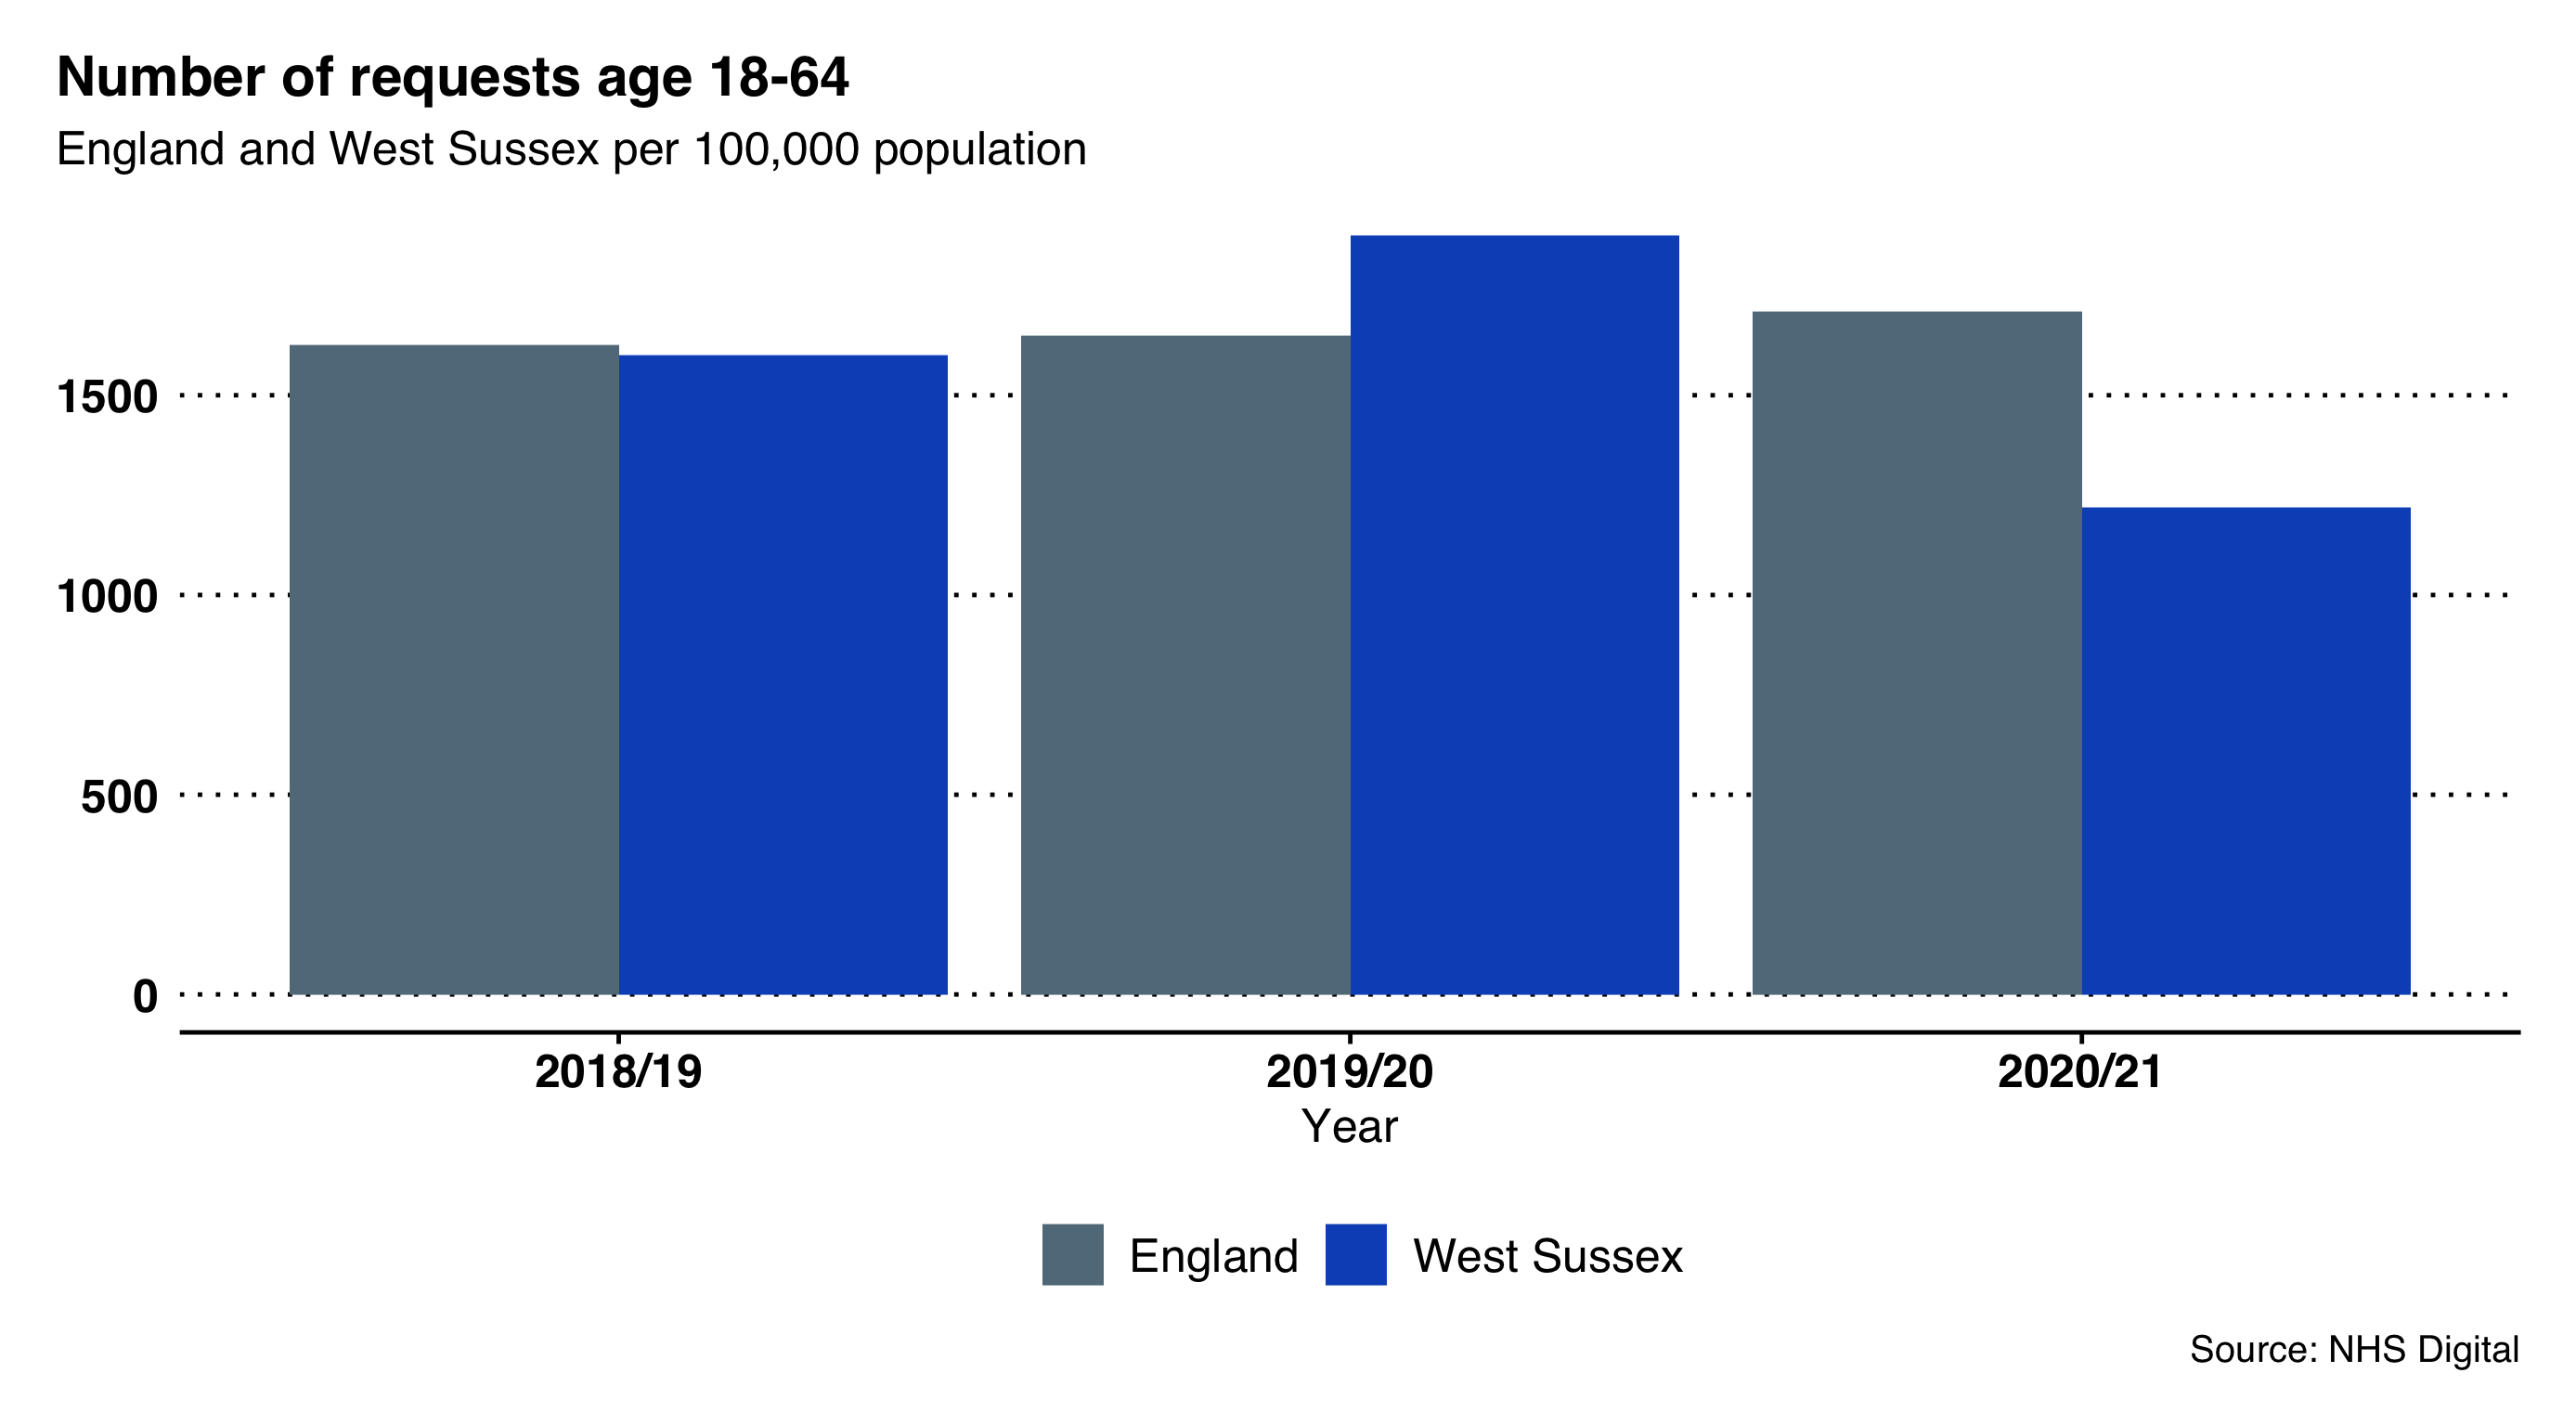
\includegraphics[width=\textwidth]{images/sc_requests_18_to_64.png}
        \caption{Number of social care requests per 100,000 population, people aged 18-64 year old, 2018/19 to 2020/21.}
        \label{fig:sc:requests_18_64}
    \end{subfigure}
    \begin{subfigure}[b]{0.49\textwidth}
        \centering
        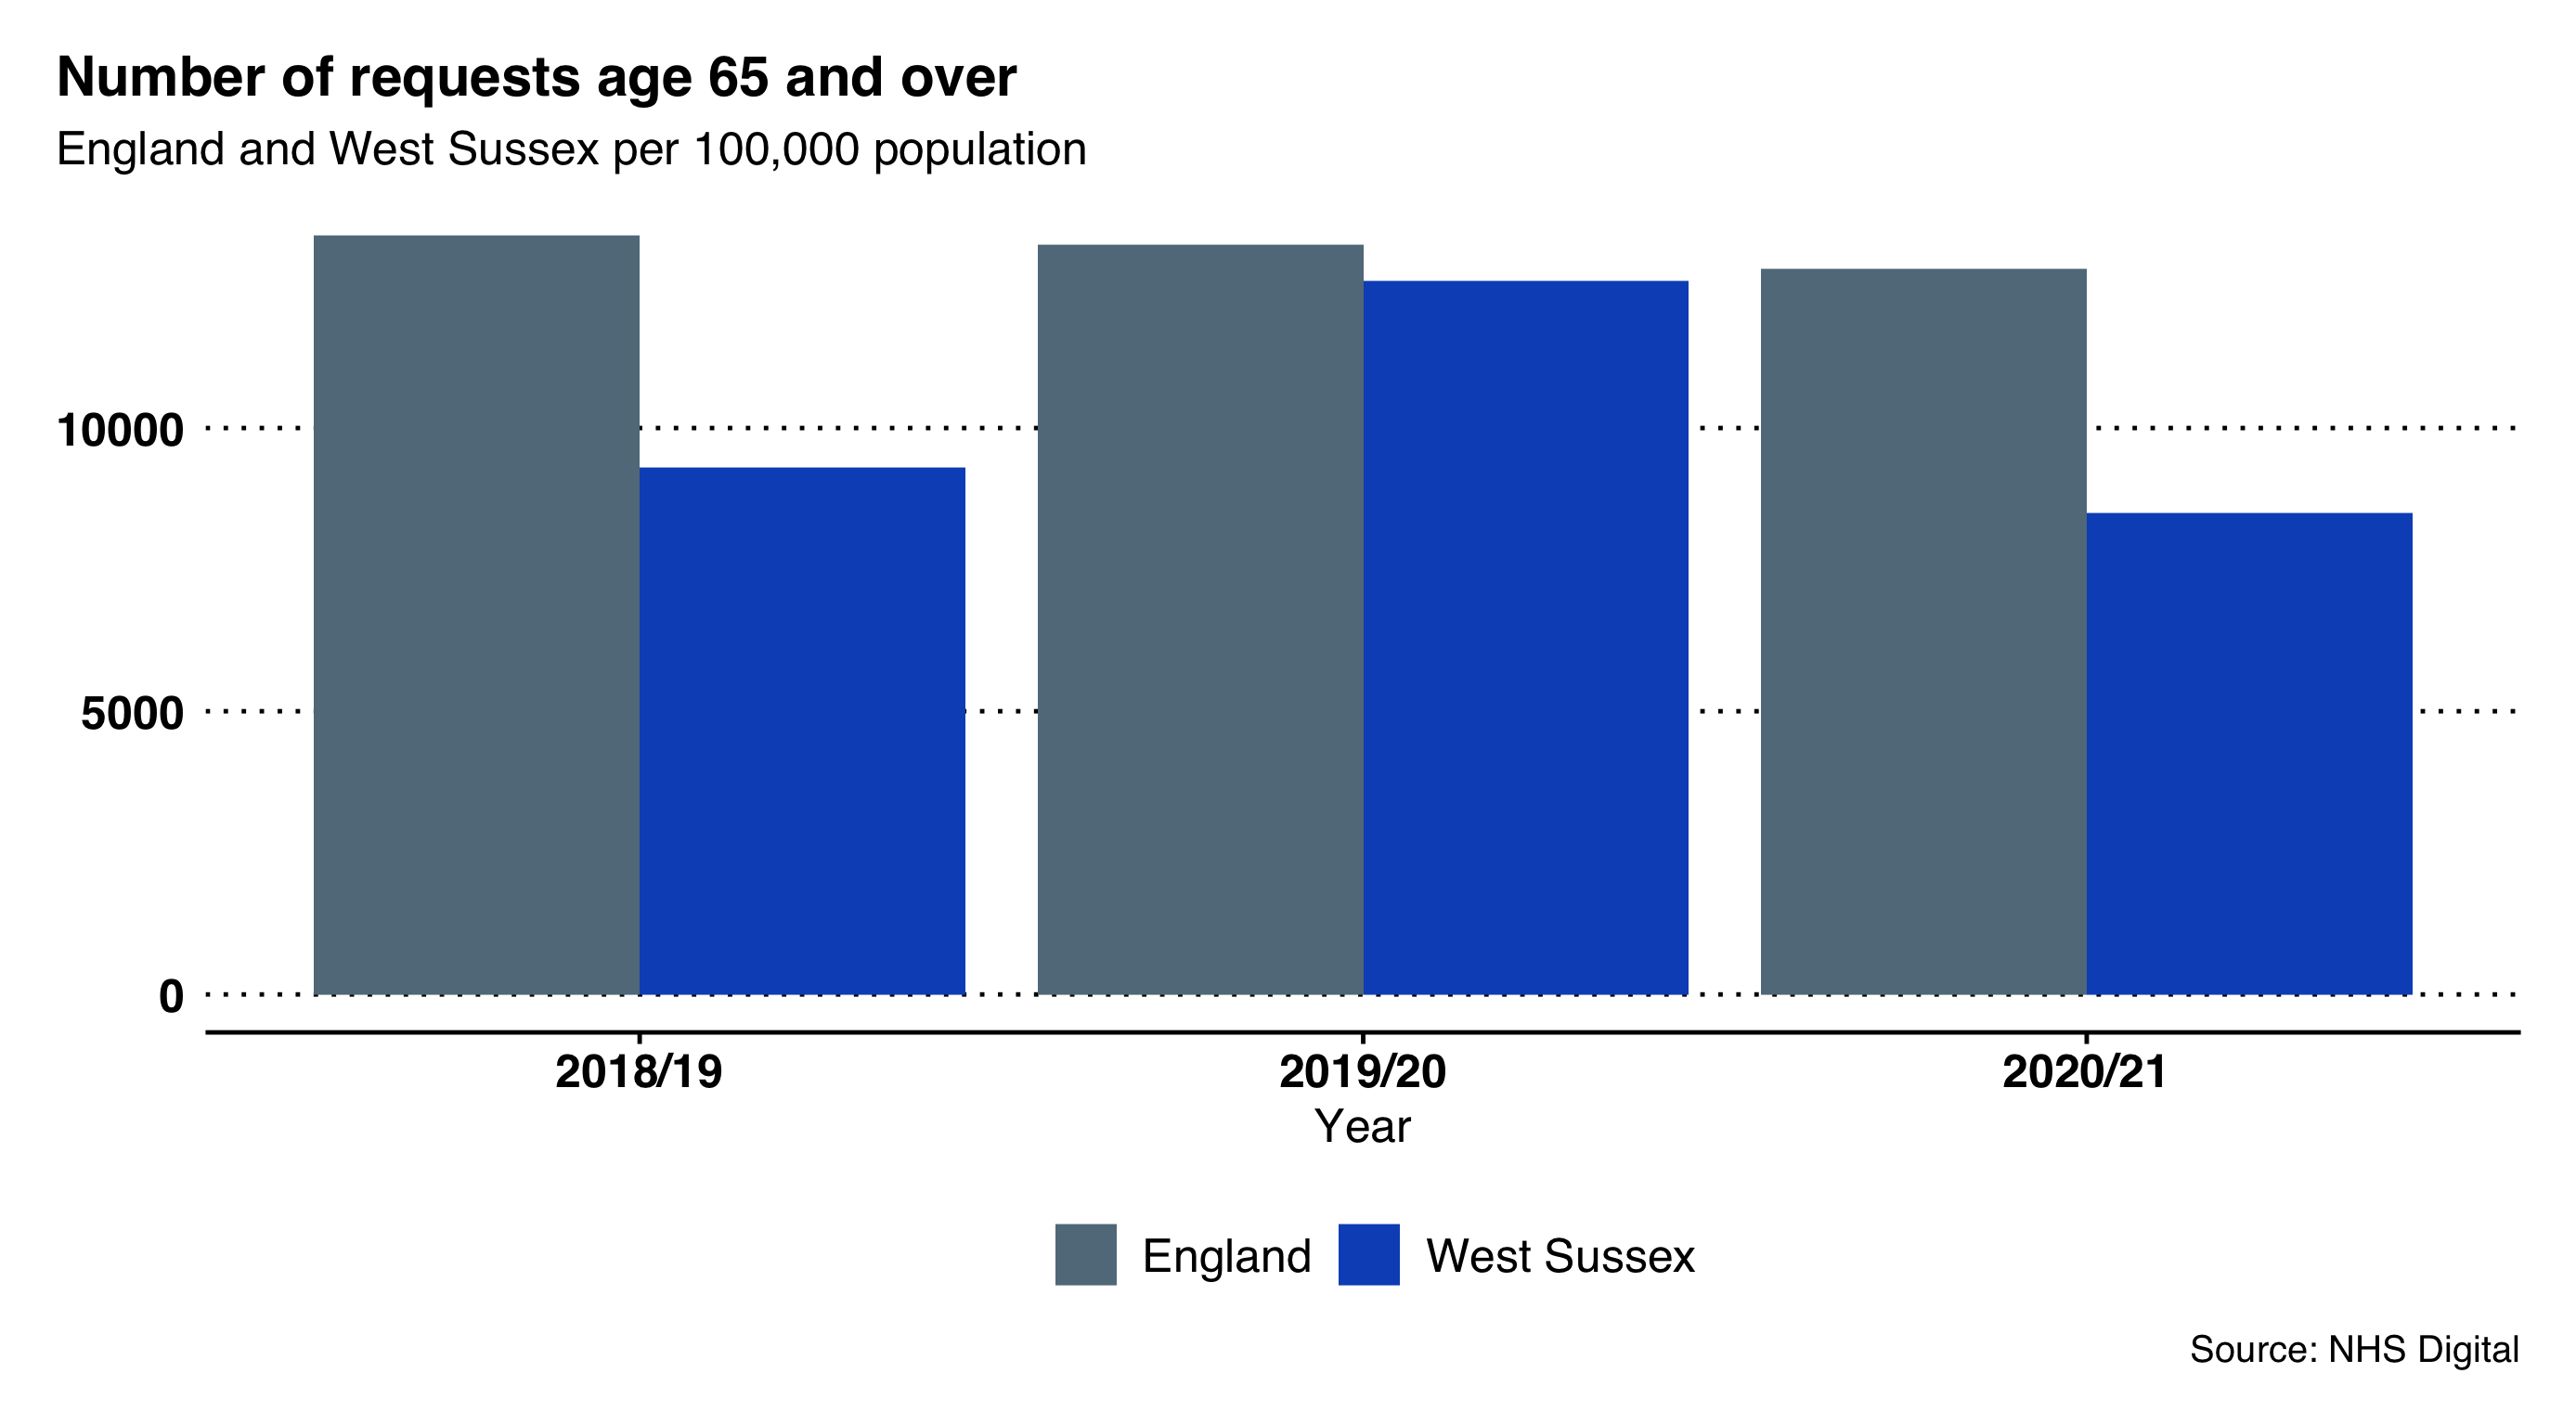
\includegraphics[width=\textwidth]{images/sc_requests_over_65.png}
        \caption{Number of social care requests per 100,000 population, people aged 65 years and over, 2018/19 to 2020/21.}
        \label{fig:sc:requests_65_plus}
    \end{subfigure}
    \begin{subfigure}[b]{0.55\textwidth}
        \centering
        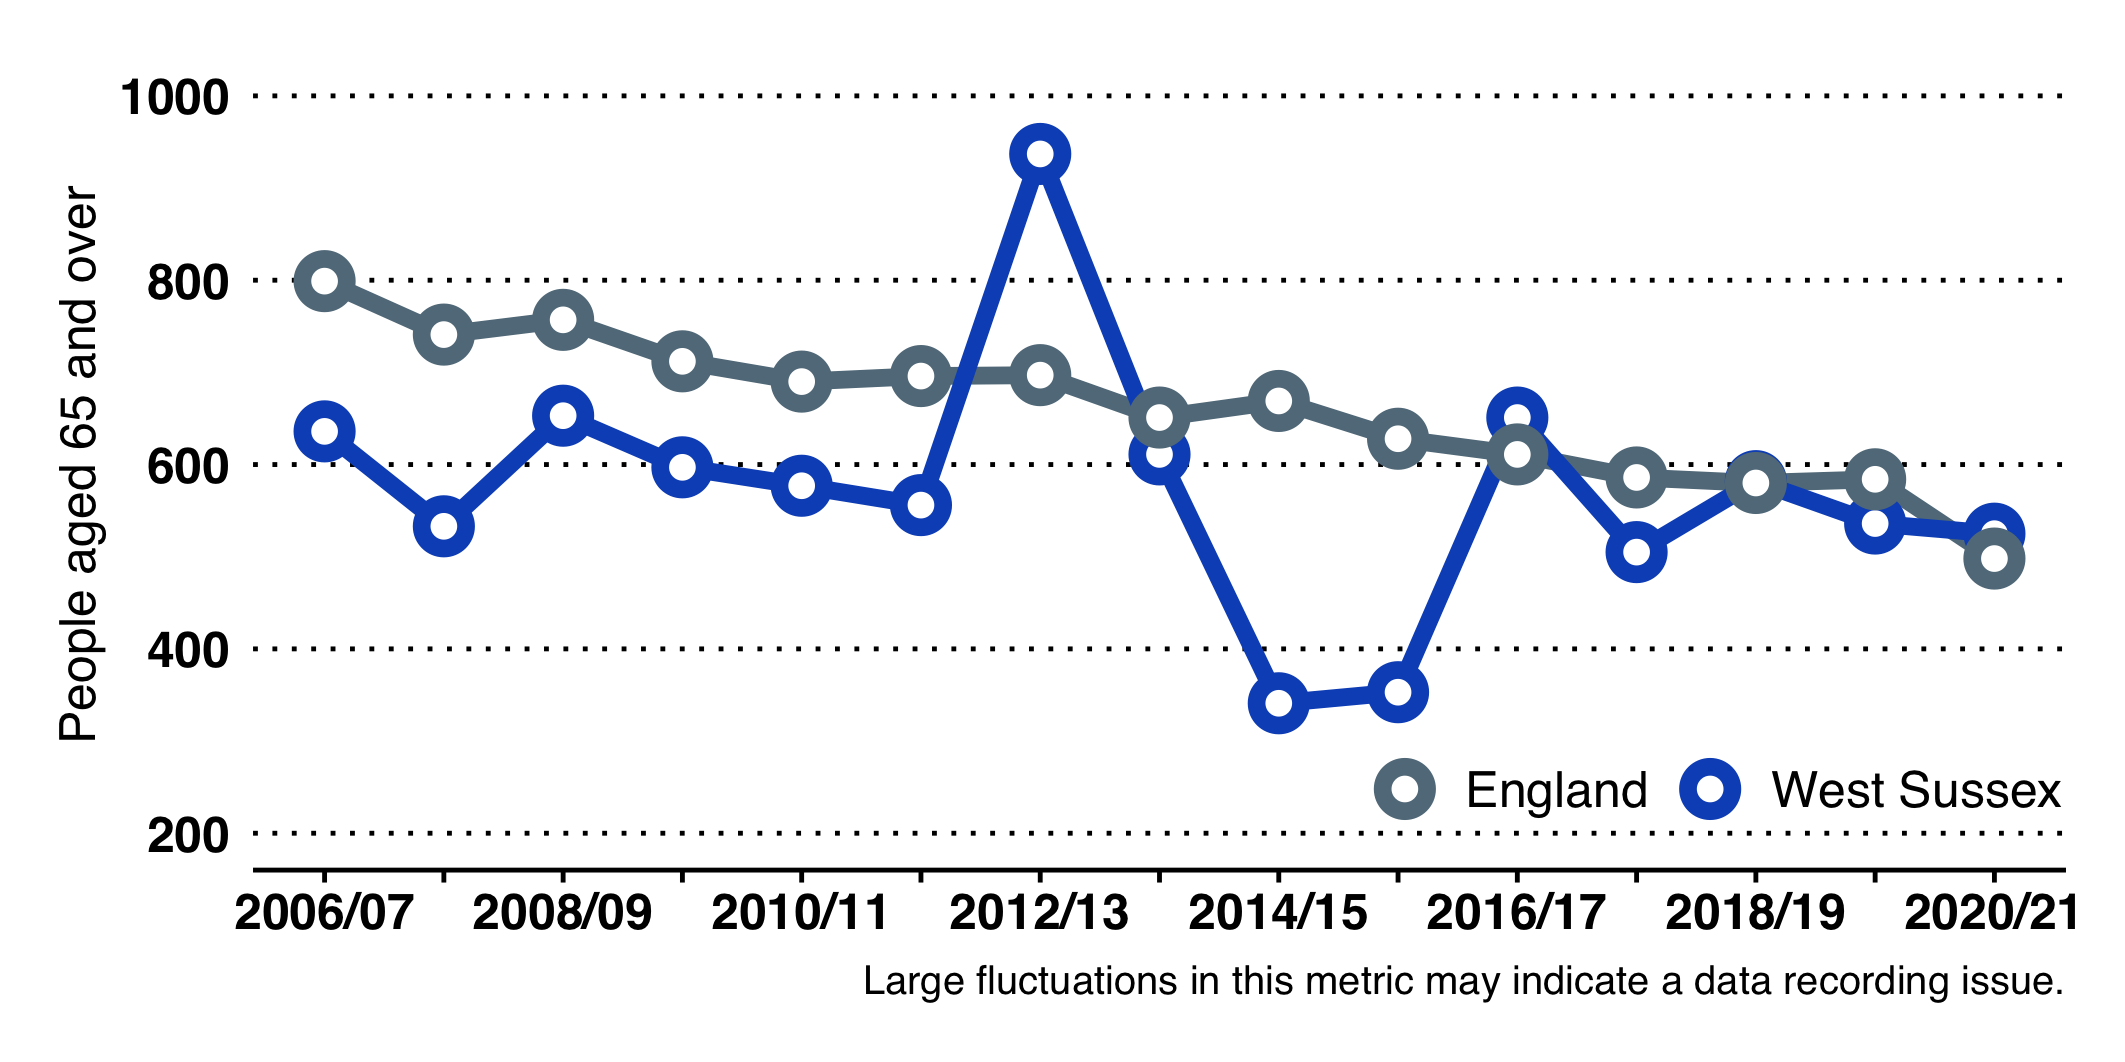
\includegraphics[width=\textwidth]{images/perm_res_adm_time.png}
        \caption{Number of permanent admissions to residential and nursing care homes per 100,000 population, West Sussex and England, 2006/07 to 2020/21.}
        \label{fig:sc:residential_admissions}
    \end{subfigure}
\end{figure*}


% FIGURE New requests from 18-64 year-olds (stacked bar by route of entry) West Sussex vs England
% FIGURE New requests from 65+ year-olds (stacked bar by route of entry) West Sussex vs England

% FIGURE Number of requests to social care by age group (line graph by age group, by time)

Data returns from WSCC to NHS Digital show a large recorded increase of requests to social care between 2016/17 and 2018/19:

\begin{itemize}[noitemsep]
    \item There were 5,965 total requests in people aged 18-64 years.
    \item In the 65+ years group, there were 17075 requests to social care.
    \item In total, there were approximately 23,000 requests for support in West Sussex in 2020/21, this is equivalent to 63 requests a day.
    \item The rate of requests, per 100,000 18-64 year-olds, is lower than the national rate.
    \item The rate per 100,000 65+ remains below that of England and comparable authorities.
    \item In West Sussex, there were 34\% fewer requests for support in working age adults (nationally these increased by 3\%) and 32\% fewer requests in those aged 65 and over (nationally these fell by 2\%).
\end{itemize}

\subsubsection{Demand over time}
\paragraph{People aged 18-64 years} The rate of new requests per 100,000 in West Sussex has increased and is now recorded as being higher than comparable authorities and England overall (see Figure~\ref{fig:sc:new_requests_18_64}).

\paragraph{People aged 65 years or over} Although the rate of new requests has increased for 65+ age group, it remains below comparable authorities and England (see Figure~\ref{fig:sc:new_requests_65_plus}).

\paragraph{Permanent admissions to residential and nursing care homes per 100,000 population} Figure~\ref{fig:sc:residential_admissions} (page~\pageref{fig:sc:residential_admissions}) shows the number of permanent admissions (of people aged 65 and over) to residential and nursing care homes per 100,000 population over time. Large fluctuations in this metric around 2012 may indicate a data recording issue.

{\bfseries In 2020/21, 1,054 people entered residential care.} Rates are similar to England and for the last five years have followed the national downward trend. West Sussex has the third highest rate of residential admissions among comparable authorities.\footnote{PHE note that: People counted as a permanent admission include: Residents where the local authority makes any contribution to the costs of care, no matter how trivial the amount and irrespective of how the balance of these costs are met; Supported residents in Local Authority-staffed care homes for residential care independent sector care homes for residential care and registered care homes for nursing care. Residential or nursing care which is of permanent nature and where the intention is that the spell of care should not be ended by set date. For people classified as permanent residents, the care home would be regarded as their normal place of residence.}

\subsection{West Sussex Social Care}
% \subsubsection{Overview of requests for support 2018-19 and the outcomes}
% NHS Digital state that there are three broad categories to group the outcomes for requests for support: short-term care to maximise independence (ST-Max), long-term care, and other support. These are shown for working age adults and older adults in this diagram.

% This diagram reflects how outcomes are classified and recorded in West Sussex. Differences from the national picture may reflect differences in interpretation.

% Note NHS Digital State: "These outcomes to a request for support can sometimes be difficult to interpret and should not be seen as reflecting negatively on a local authority, but more as a statement about the nature of request for support that was made."

% FIGURE - flow chart for people aged 18-64 versus people aged 65 and over

% Fewer outcomes in West Sussex are classified as ST-Max, and there is also a lower percentage of long term support. Of the "other" subdivision, West Sussex also has a lower percentage receiving no services, with a far higher proportion being signposted to universal or other services.

% As with the working age group, fewer outcomes of ST-Max are being recorded. A similar percentage are going onto long term support. A higher percentage of requests are recorded as being signposted to universal or other services. It is noted that no outcomes are recorded as being NHS-funded care or end of life care.

% (probably best to crib off the original page and data I was able to grab off NHS Digital)

\subsubsection{ASCOF Outcomes and the Adult Social Care Users Survey 2020-21}
Each year a sample of people in receipt of support that is funded or managed by social services are surveyed. The survey asks a range of questions, such as how satisfied people are with the support provided and how the support affects their lives. The survey has a variety of questions but here we only show results relating to overall satisfaction, social contact and access to information.

However, the 2020-21 Adult Social Care Users Survey was voluntary. As only 18 CASSRs participated in the 2020-21 survey, aggregated ASCOF outcomes have not been calculated at regional, council type and England level. West Sussex was not one of those CASSRs.

\subsection{Falls and Fractures}
\paragraph{Falls People Aged 65 years or over} Falls in later life are one of the key triggers for entry into residential care. Key risk factors are age and sex. Older people with dementia and sensory impairment are more likely to experience a fall.

The rate of emergency hospital admissions as a result of a fall is relatively high in West Sussex, and of particular concern is the higher rate amongst the 80+ years age group. In 2020/21, the rates were:

\begin{itemize}[noitemsep]
    \item People aged 65+ years\footnote{PHOF reference C29} - 2,280 per 100,000 (4,965 falls) (England rate, 2,023). Broken down:
    \begin{itemize}[noitemsep]
        \item People aged 65-79 years - 1,016 per 100,000 (1,460 falls) (England rate, 937)
        \item People aged 80+ years 5,946 per 100,000 (3,505 falls) (England rate, 5,174)
    \end{itemize}
\end{itemize}

\paragraph{Hip Fractures - People Aged 65 years or over} Hip fractures are of particular concern. Public Health England state that one in three older people who have a hip fracture return to their former levels of independence but one in three ends up moving into long-term residential or nursing care. In 2018/19, the rates were:

\begin{itemize}[noitemsep]
    \item People aged 65+ years\footnote{PHOF reference E13} - 532 per 100,000 (1,160 hip fractures) (England rate, 529). Broken down:
    \begin{itemize}[noitemsep]
        \item People aged 65-79 years - 225 per 100,000 (325 hip fractures) (England, 219)
        \item People aged 80+ years - 1,422 per 100,000 (835 hip fractures) (England, 1,426)
    \end{itemize}
\end{itemize}

% Would be nice to revisit this table in a future summary
% \begin{table*}
%     \caption{Odds ratio (Falls v Not Falls) of non-elective admissions of 65 years and over West Sussex CCG responsibility 2013/14 to 2017/18 (5 years pooled data)}
%     \centering
%     \begin{tabular}{llllll}
%         \toprule
%         Description & ICD Coding & Number with Falls & Odds Ratio & LCI & UCI \\
%         \midrule
%         Eye disorders & ICD-10 H00 - H58 & 3,862 & 1.4 & 1.4 & 1.5 \\
%         Vestibular disorders & ICD-10 H81 & 147 & 1.2 & 1 & 1.4 \\
%         Hearing loss & ICD-10 H90 - H91 & 1,745 & 1.9 & 1.8 & 2 \\
%         Dementia & ICD-10 F00 to F03, G30 & 7,489 & 2.2 & 2.2 & 2.3 \\
%         \bottomrule
%     \end{tabular}
%     \label{tab:op:f_vs_nf}
% \end{table*}

% \begin{tcolorbox}[colback={boxcolour},title={Key risk factors}]
%     \begin{itemize}[noitemsep]
%         \item Age and sex
%         \item Older people with dementia and sensory impairment
%     \end{itemize}
% \end{tcolorbox}
    
% \subsubsection{Emergency Admissions for Falls - Age and Sex Profile} The graph below has combined 5 YEARS OF HOSPITAL DATA (2013/13 to 2017/18), showing emergency admissions of people aged 65 years or over by age group and sex (graphs)

% FIGURE - Emergency Admissions for Falls - Age and Sex Profile

\subsubsection{Vaccination coverage in over-65s}
The coverage of the PPV vaccination in over-65s\footnote{PHOF reference D06b} was 71.5\% in 2020/21, in line with England and CIPFA neighbours.

The coverage of the flu vaccine for people aged 65 years and over\footnote{PHOF reference D06a} in 2020/21 was 83.7\% in 2018/19. This is above the 75\% benchmark, and higher than the England coverage (81\%) and the average of CIPFA neighbours.

The success of the Covid-19 vaccination programme has likely had a positive effect on the uptake of flu vaccination in over 65s.

\begin{figure}
    \caption{Proportion of population aged 65 or over receiving a flu vaccination, West Sussex and England 2010/11 to 2020/21.}\label{fig:over65fluvax}
    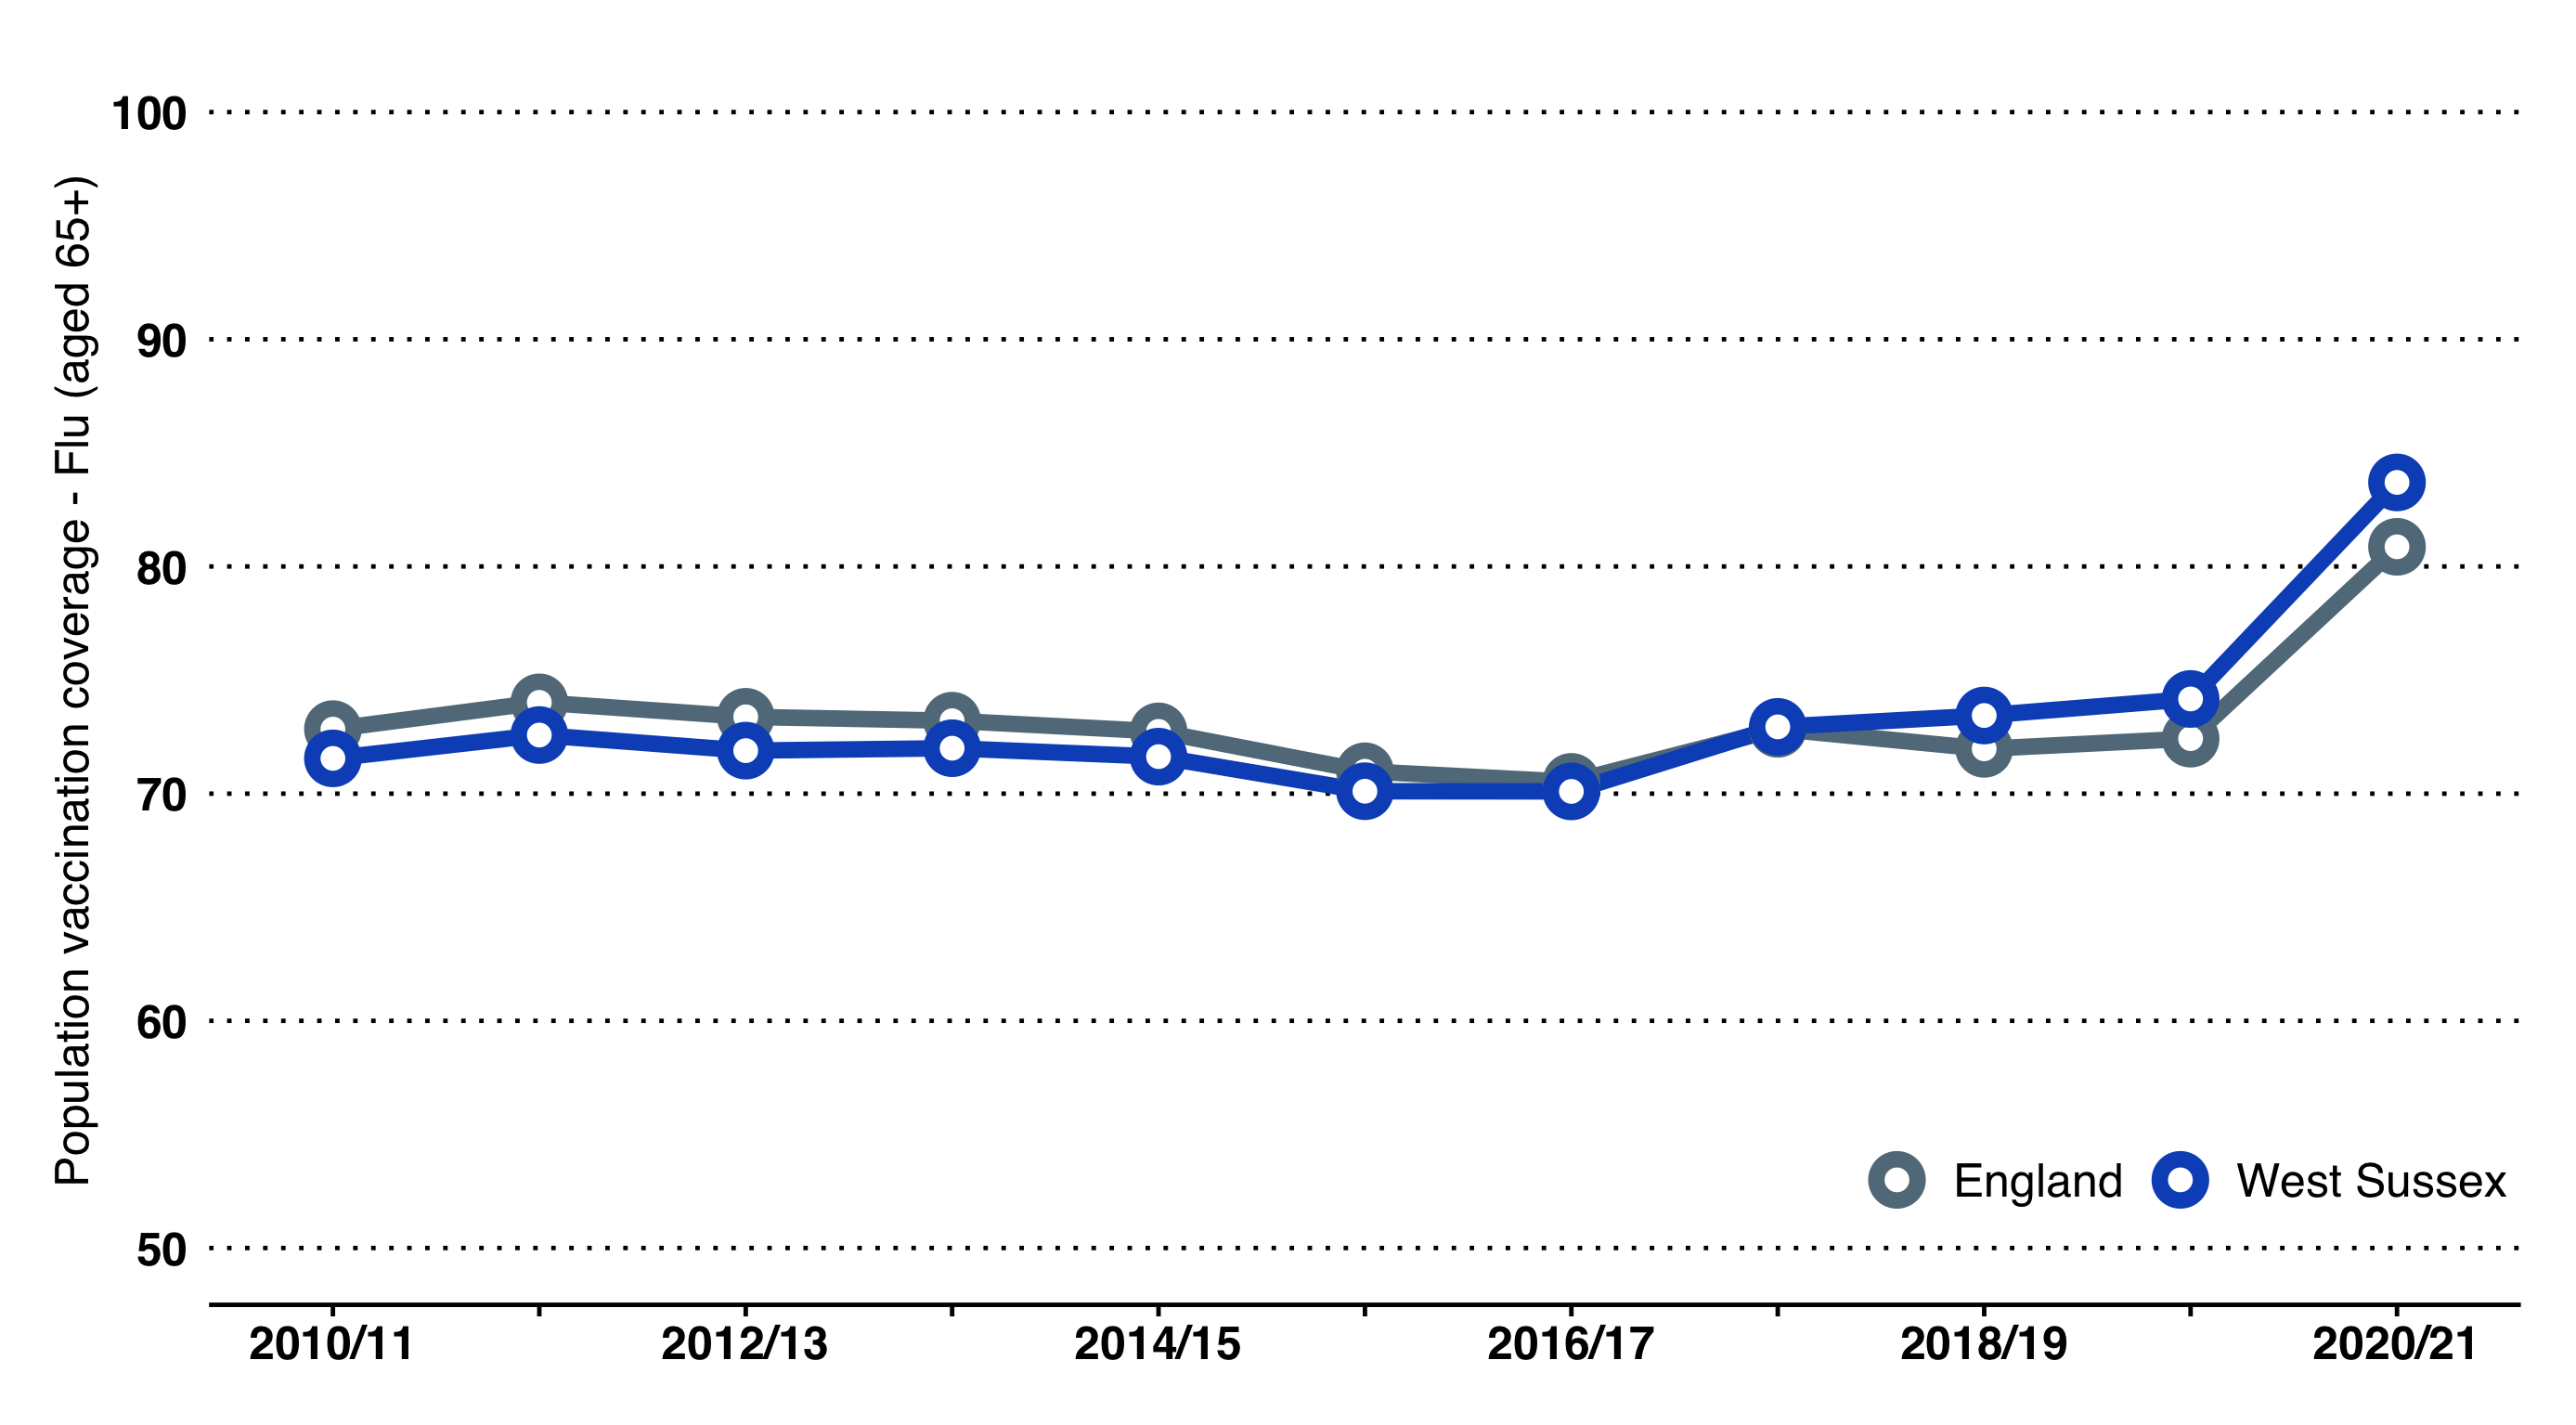
\includegraphics[width=\linewidth]{images/65over_vaccine_flu.png}
\end{figure}

% \subsection{A Focus on EMERGENCY ADMISSIONS}
% In 2018, the National Audit Office published the report "Reducing Hospital Admissions"\footnote{https://www.nao.org.uk/report/reducing-emergency-admissions/} which took a whole system approach to action aimed at reducing the impact of emergency admissions on acute hospitals. Part one of this report focused on national trends in emergency admission.

% The Public Health and Social Research Unit now has access to Hospital Episode Statistics and so has, where possible, recreated and updated this analysis for the registered population of the three CCGs in West Sussex. This analysis looked at 5 years of data.

% A summary is shown over the next 3 pages; the full briefing is available on the JSNA website. Contact Dr Lesley Wilkes (\url{lesley.wilkes@westsussex.gov.uk}) for further information.

% Note: Analysis is based on the registered population, i.e. people who are registered with a West Sussex GP.

% \subsubsection{Key Points}
% Emergency admissions increased each year between 2013/14 and 2017/18. In 2013/14, there were 81,200 admissions, rising to 94,000 admissions in 2017/18, which represents an increase of 16\% over this period. In 2017/18, 17.6\% of admissions of West Sussex residents were considered to be avoidable.

% A large proportion (62\%) of the growth in emergency admissions (completed spells) from 2013/14 to 2017/18 was accounted for by people who did not stay overnight.

% In 2017/18, nearly half of admissions (49\%) resulted in stays of two or more nights. 31\% of people admitted did not stay overnight.

% Older people (65 years and over) made up 60\% of the growth in emergency admissions between 2013/14 and 2017/18. Some of this is due to demographic changes: between 2013/14 and 2017/18 the number of people aged 65 and over in the registered population of West Sussex grew by 12,850, an increase of 7\%. Over the same period, the number of emergency admissions to those aged 65+ grew by 7,700, an increase of 19\%.

% \begin{table}
%     \caption{Number and rate of emergency admissions. All ages, West Sussex, 2013/14 to 2017/18.}
%     \centering
%     \begin{tabular}{lll}
%         \toprule
%         Year & Number & Rate per 1,000\footnote{Registered population}\\
%         \midrule
%         2013/2014 & 81,186 & 95.72 \\
%         2014/2015 & 82,660 & 96.24 \\
%         2015/2016 & 87,624 & 101.05 \\
%         2016/2017 & 91,825 & 104.63 \\
%         2017/2018 & 94,003 & 106.15 \\
%         \bottomrule
%     \end{tabular}
%     \label{tab:op:em_adms}
% \end{table}

% The number of bed days decreased between 2013/14 and 2017/18, from 566,150 to 505,050, a decrease of 11\%. Whilst the number of emergency admissions resulting in 0, 1, or 2+ days has increased, the average length of stay of those admitted for 2 or more nights has decreased, from 12.2 days in 2013/14 to 10.1 days in 2017/18.

% The number of available beds increased between 2013/14 and 2017/18 for each of the three main trusts that serve West Sussex. The number of occupied beds also increased in all three trusts.


% \subsubsection{The Story in Tables and Charts...} Number and rate of emergency admissions in West Sussex, 2013/14 to 2017/18 Overall, emergency admissions of West Sussex residents have increased year-on-year. In 2013/14, there were 81,200 non-elective admissions (all ages); by 2017/18 this had risen to 94,000, representing a 15.8\% increase (12,800 more admissions). Over this period the population of West Sussex has also increased, by 4.4\%; when expressed as a rate per 1,000, emergency admissions still demonstrated an increase, but of a lower percentage, at 10.9\%.

% FIGURE - Number of emergency admissions by age group 2013/14 and 2017/18

% FIGURE - Change in number of emergency admissions by age group 2013/14 to 2017/18

% FIGURE - Rate per 1,000 of emergency admissions by age group 2013/14 and 2017/18

% FIGURE - Change in rate per 1,000 of emergency admissions by age group 2013/14 to 2017/18

% The largest increases in the number of emergency admissions are amongst the very young (0-4 years) and the older population (70+ years), especially the very old (85+).

% Note: the large increase in the number of admissions for the 70-74 years group reflects the underlying demographic increase in this age group.

% The largest increases in the rate of emergency admissions are also in the very young (0-4 years) and elderly population (80+).

% \subsubsection{Bed days}
% While the number of completed spells has increased over the period 2013/14 to 2017/18, reflecting the increase in the number of emergency admissions, the number of bed days has decreased, from 566,150 to 505,100 (a decrease of 11\%).

% There was a large drop in the number of bed days between 2013/14 and 2014/15, and maintenance of this lower level to 2017/18.

% A completed spell is the total period a person spends in hospital from admission to discharge. Not everyone admitted will spend a day in hospital, as they may be discharged within the day.

% \begin{table*}
%     \caption{Completed spells, Length of Stay (LoS), and Average Length of Stay (2013/14 to 2017/18)}
%     \centering
%     \begin{tabular}{lrrrrr}
%         \toprule
%         \ & 2013/14 & 2014/15 & 2015/16 & 2016/17 & 2017/18 \\
%         \midrule
%         Number of & 85,500 & 85,350 & 91,500 & 96,150 & 98,650\\
%         completed spells & \ & \ & \ & \ & \ \\
%         Total bed days & 566,150 & 509,900 & 513,950 & 512,200 & 505,100\\
%         Stays of 0 Days & 22,050 & 22,200 & 24,850 & 28,150 & 30,200\\
%         Stays of 1 Day & 18,550 & 18,950 & 20,500 & 20,350 & 20,400\\
%         Stays of 2+ Days & 44,900 & 44,200 & 46,150 & 47,650 & 48,000\\
%         Total no. bed days & 547,600 & 490,950 & 493,450 & 491,850 & 484,700\\
%         with 2+ days LoS & \ & \ & \ & \ & \ \\
%         Average stay of & 12.2 & 11.1 & 10.7 & 10.3 & 10.1\\
%         long stays & \ & \ & \ & \ & \ \\
%         (2+ days) & \ & \ & \ & \ & \ \\
%         \bottomrule
%     \end{tabular}
%     \label{tab:op:bed_days}
% \end{table*}

% \paragraph{Bed usage differs with age...} People 65+ years accounted for about 50\% of the finished emergency spells in 2017/18, despite comprising only 22\% of the registered population.

% Over-65s also use a greater proportion of the bed days (74\% of bed days).

% FIGURE - Stacked bar graph showing age groups and duration of stay (emergency admissions vs emergency bed days)

% {\bf Change in Emergency Admissions by Type of Patient (2013/14 to 2017/18)}
% Emergency admissions have risen for each of the four patient groups examined (see key), and by more than would be accounted for by demographic change.

% Admissions for all ages, those aged 65 years and over, and those considered avoidable rose by a similar percentage (14-19\%), although there was a slight drop in the number of avoidable admissions between 2016/17 and 2017/18.

% Emergency admissions for those at risk of frailty, however, increased at a much faster rate between 2015/16 and 2017/18 and were a third higher in 2017/18 than in the base year 2013/14.

% For each group of patients, the number of admissions in 2013/14 was taken to be 100\%, and the number in subsequent years expressed as a percentage of this.

% FIGURE - Change in Emergency Admissions by Type of Patient (2013/14 to 2017/18)
\subsection{Mortality}
\subsubsection{Underlying Cause of Death} In 2020, there were approximately 10,100 deaths. Cancer and diseases of the circulatory and respiratory systems account for 60\% of all deaths.

For underlying cause of Death in Figure~\ref{fig:underlying-cod}, we use ICD-10 chapter headings for broad underlying cause of death. Note that deaths from Covid-19 were classified with new codes and these come under the chapter heading "New and Special codes".

\begin{figure}
    \caption{Underlying cause of death, West Sussex 2020}\label{fig:underlying-cod}
    \centering
    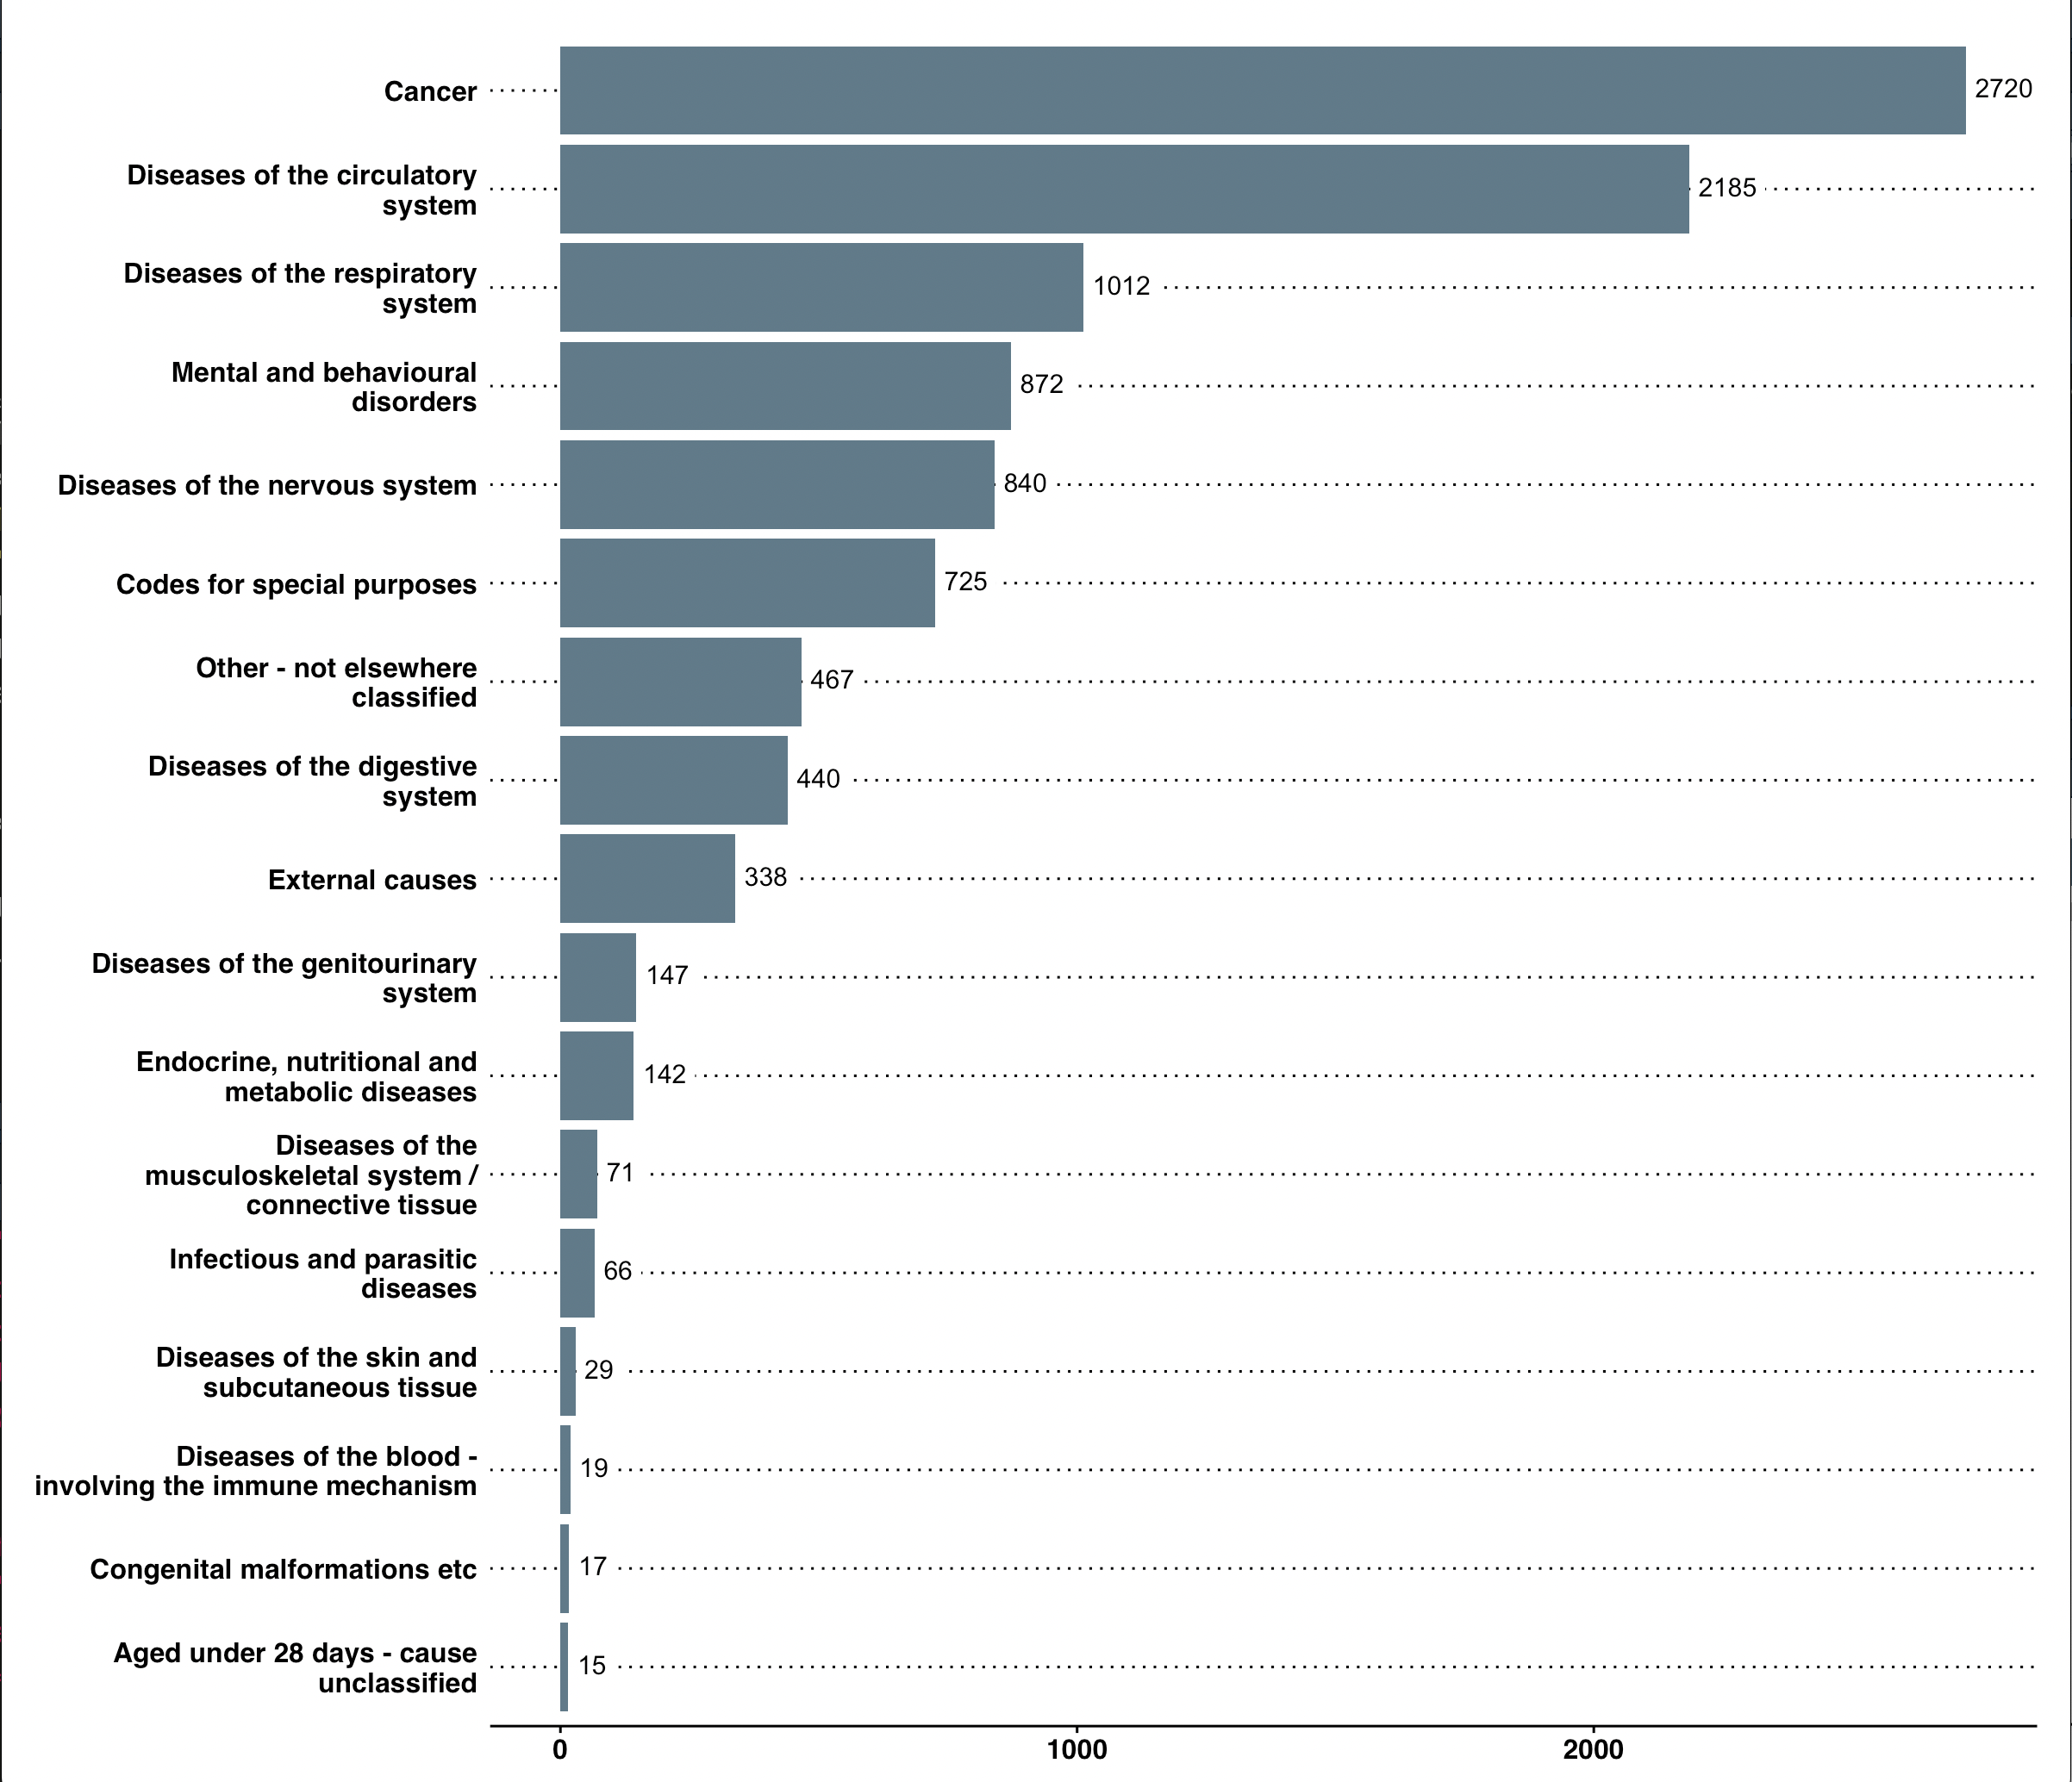
\includegraphics[width=\linewidth]{images/underlying_cause_of_death.png}
\end{figure}

\subsubsection{Place of Death}

 In the absence of other measures, the place of death is often used as a proxy for the quality of end of life care. This reflects the fact that, when asked, many people express a preference to die in their own home surroundings, or supported in a hospice, rather than a hospital setting.

 PHE produce annual Palliative and End of Life Care Profiles, but these have not been updated with local data since 2019. Note that the figures in Figure~\ref{fig:DiUPR} are from 2017. As noted in the previous  JSNA summary: {\textit "In West Sussex, there is a considerable difference between local authorities. In Crawley, 40.3\% of people died at their usual place of residence, which was the lowest percentage in the South East region, whilst Chichester had the highest percentage in the region, at 58.3\%."}

\begin{figure}
    \caption{Proportion of deaths occurring in the usual place of residence, West Sussex and local authorities, 2017.}\label{fig:DiUPR}
    \centering
    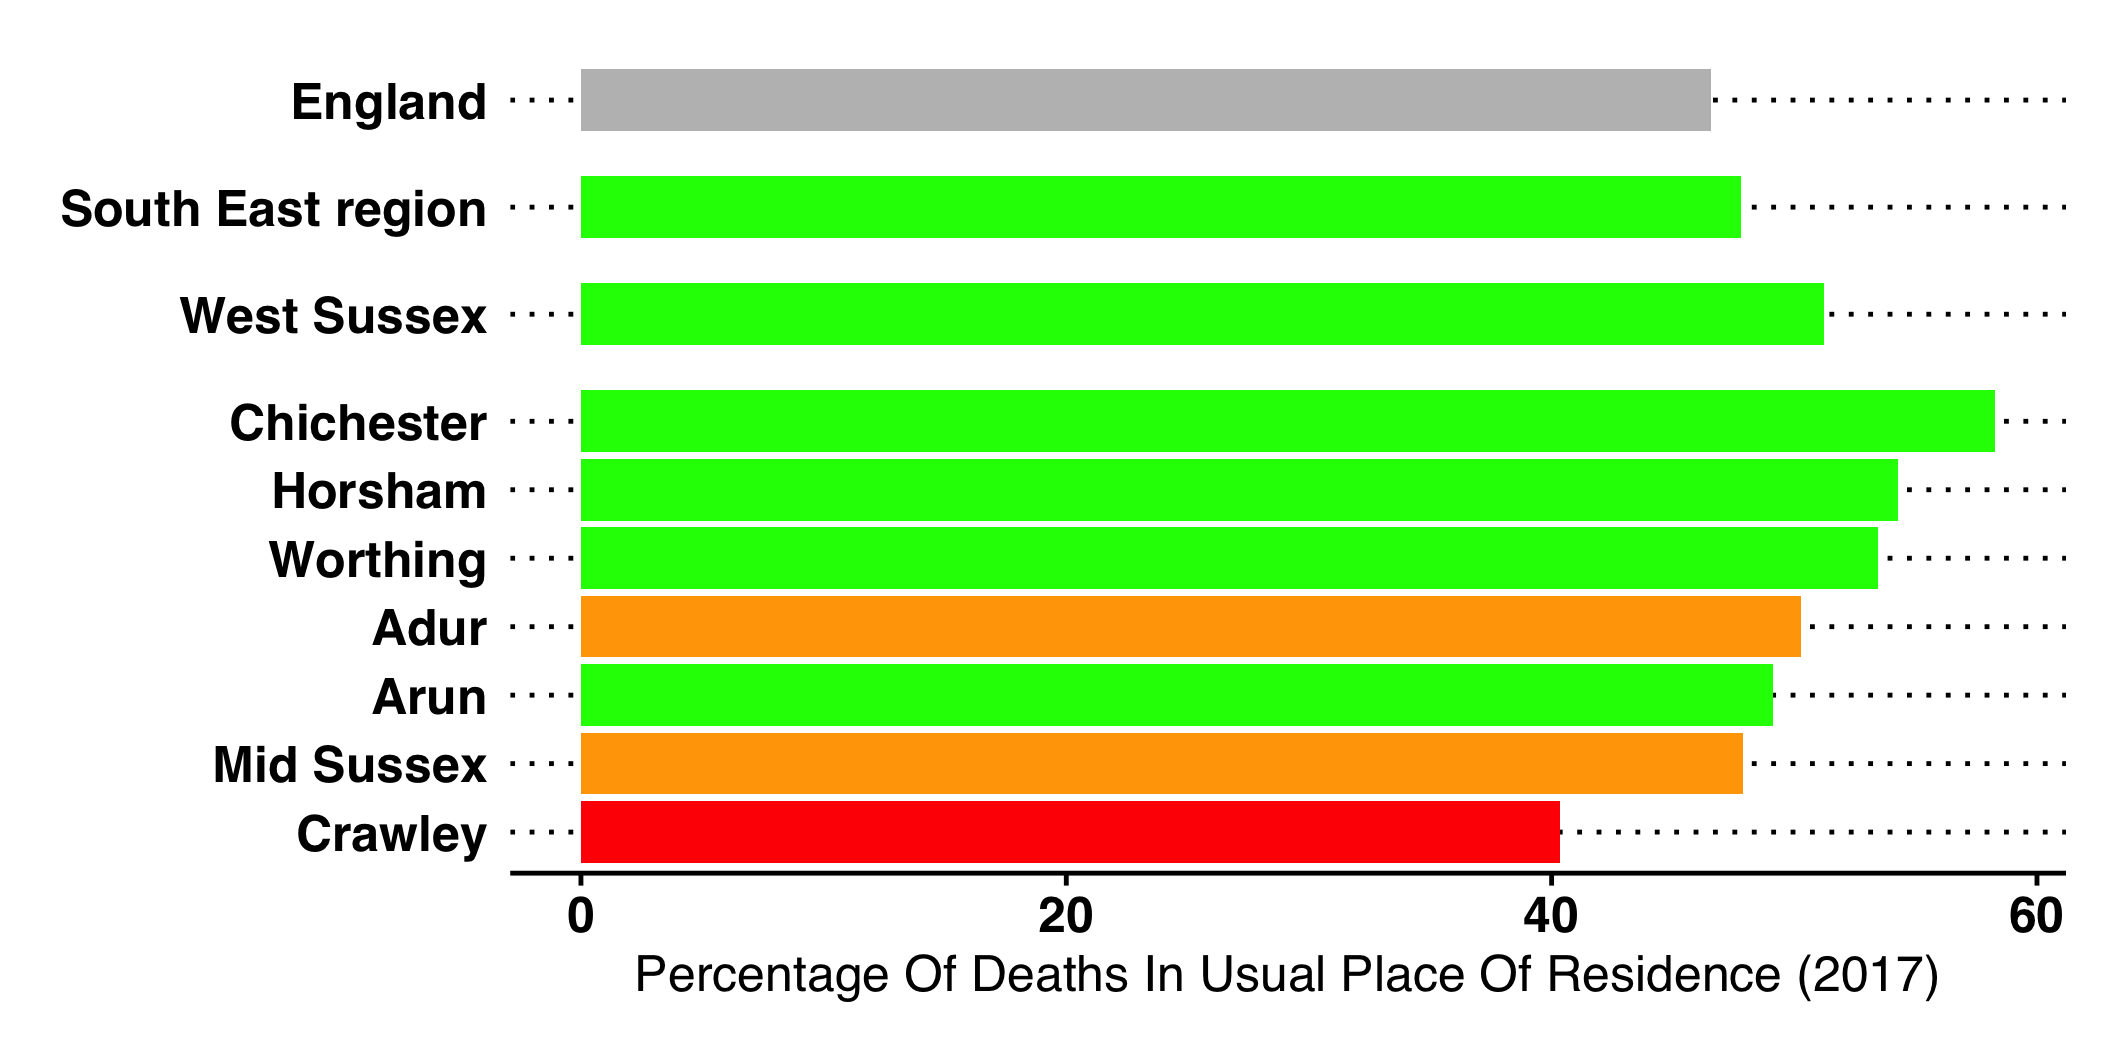
\includegraphics[width=\linewidth]{images/diupr_rag_bar.png}
\end{figure}

\subsubsection{Excess Winter Deaths}
The Excess Winter Deaths Index (EWD Index)\footnote{PHOF reference E14. Note that 2020 figure excludes deaths from Covid-19. ONS also provide estimates  inclusive of Covid-19 deaths.} is the ratio of extra deaths from all causes that occur in the winter months compared with the expected number of deaths, based on the average of the number of non-winter deaths. 

\begin{table}
    \caption{West Sussex Excess Winter Deaths. An asterisk indicates periods when excess winter deaths in West Sussex were significantly higher than England.}
    \centering
    \begin{tabular}{lll}
        \toprule 
        \ & Excess ratio & Number \\
        \midrule
        Aug 2001 - Jul 2002 & 19.2 & 568 \\
        Aug 2002 - Jul 2003 & 12.8 & 376 \\
        Aug 2003 - Jul 2004 & 13.5 & 392 \\
        Aug 2004 - Jul 2005 & 17.6 & 499 \\
        Aug 2005 - Jul 2006 & 20.0 & 556 \\
        Aug 2006 - Jul 2007 & 17.6 & 487 \\
        Aug 2007 - Jul 2008 & 12.2 & 342 \\
        Aug 2008 - Jul 2009 & 23.7 & 644 \\
        Aug 2009 - Jul 2010 & 17.0 & 457 \\
        Aug 2010 - Jul 2011 & 21.7 & 570 \\
        Aug 2011 - Jul 2012 & 26.0* & 688* \\
        Aug 2012 - Jul 2013 & 17.2 & 473 \\
        Aug 2013 - Jul 2014 & 10.6 & 284 \\
        Aug 2014 - Jul 2015 & 29.8 & 843 \\
        Aug 2015 - Jul 2016 & 14.3 & 409 \\
        Aug 2016 - Jul 2017 & 28.9* & 815* \\
        Aug 2017 - Jul 2018 & 35.4 & 997 \\
        Aug 2018 - Jul 2019 & 15.4 & 430 \\
        Aug 2019 - Jul 2020 & 14.9 & 440 \\
        \bottomrule
    \end{tabular}
    \label{tab:op:exwd}
\end{table}
 
Looking at a longer period of time at a county level, we can see that the mean number of excess winter deaths in West Sussex is 574. In some years, deaths have been as high as 1,000 (in 1997) and as low as 280 (2014).

Figure~\ref{fig:ewd_control_chart} shows the number of excess deaths in each year since 1992. The black line shows the long term mean. The red lines represent the upper limits to the data (the dotted line being one standard deviation (SD) from the mean, and the solid red line being 2 SDs). The green lines show the lower limits. In 1997, 2000, and 2018 the number of excess deaths were unusually high.

\begin{figure}
    \caption{Control chart of excess winter deaths in West Sussex, 1992 to 2020}\label{fig:ewd_control_chart}
    \centering
    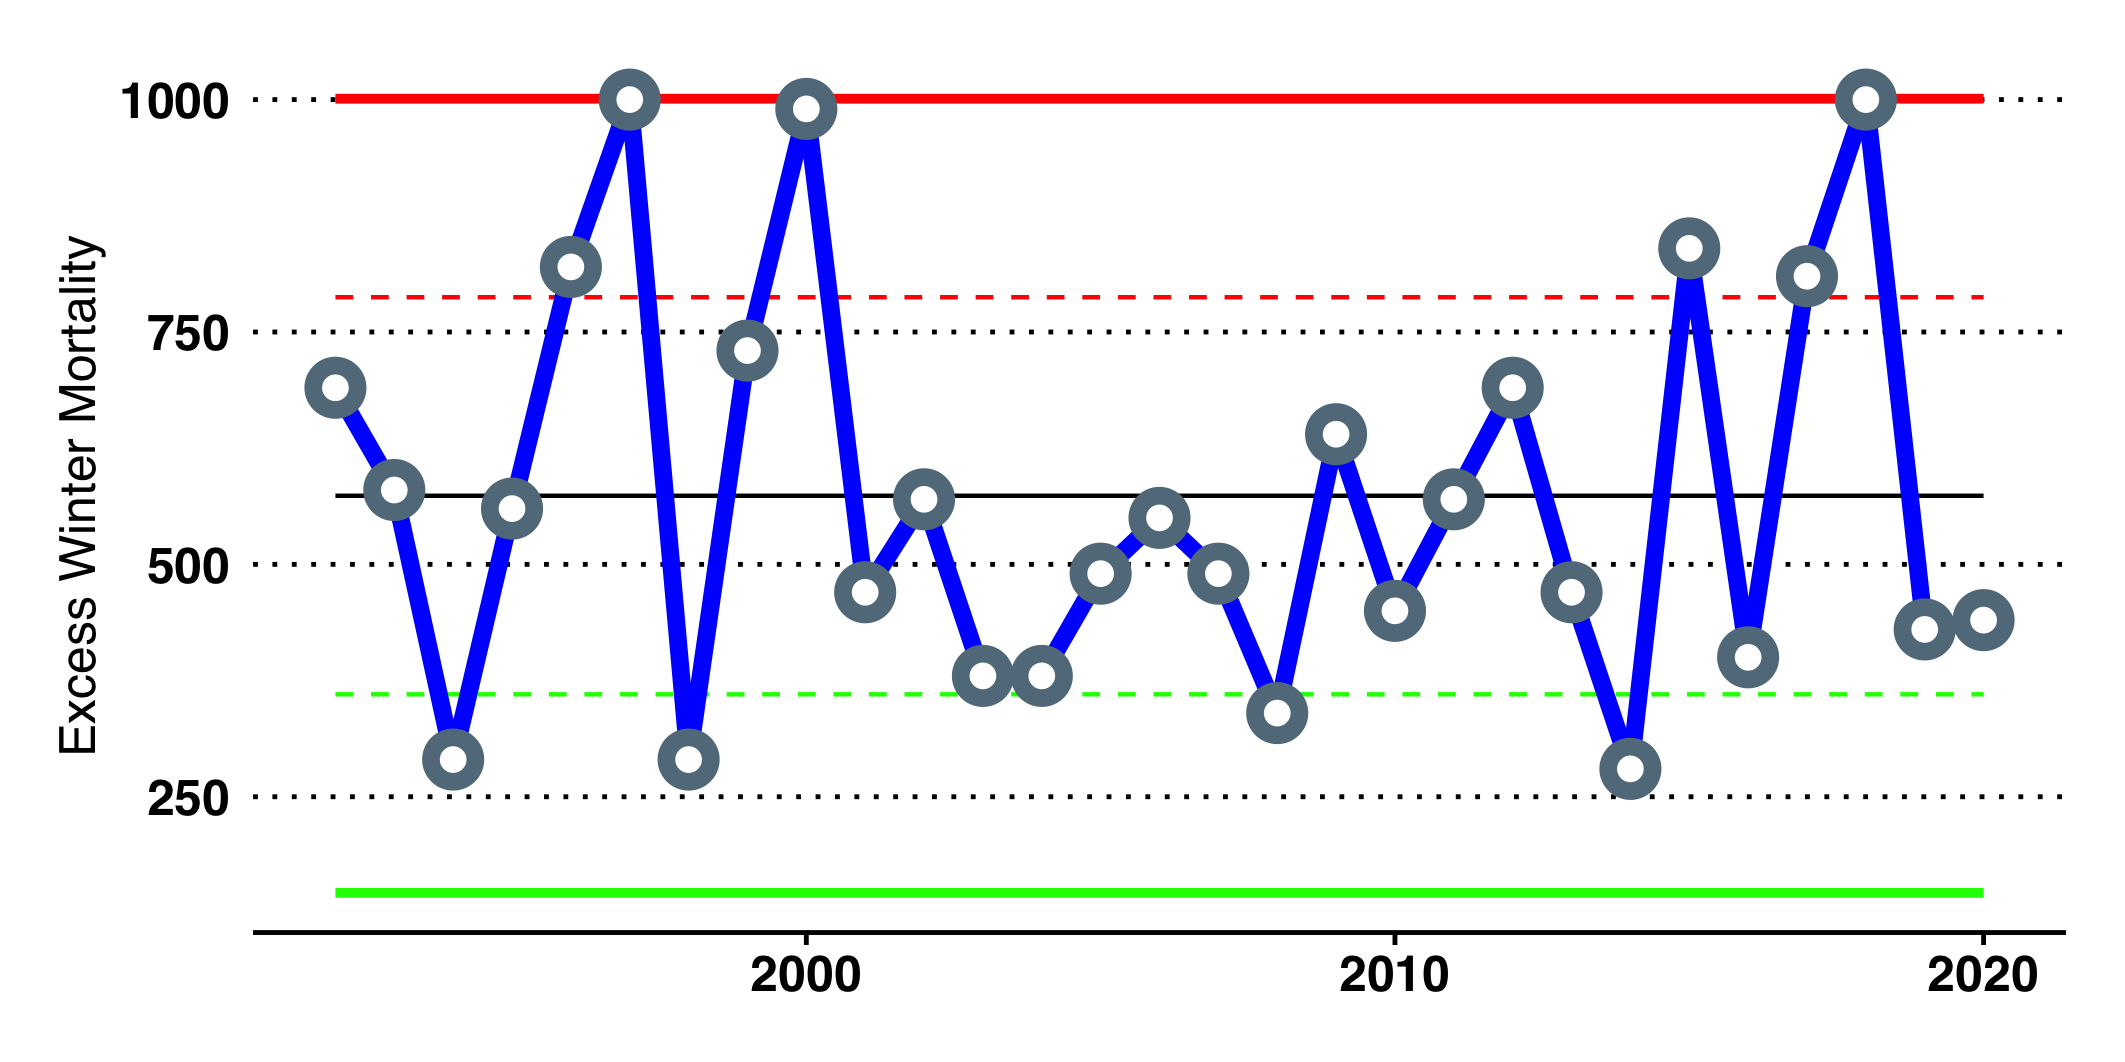
\includegraphics[width=\linewidth]{images/ewd_control_chart.png}
\end{figure}

% \subsection{Further Information}
% This is a summary document; more detailed local analyses (alongside a whole host of national profiles!) are available, including the needs assessment and briefings highlighted below. If you have specific information requests please contact the team.

% Contacts in the West Sussex Public Health and Social Research Team for Ageing Well: 
% \begin{itemize}[noitemsep]
%     \item Jacqueline Clay - (\url{jacqueline.clay@westsussex.gov.uk})
%     \item Dr Richard Tyler - (\url{richard.tyler@westsussex.gov.uk})
% \end{itemize}